% Options for packages loaded elsewhere
\PassOptionsToPackage{unicode}{hyperref}
\PassOptionsToPackage{hyphens}{url}
%
\documentclass[
]{article}
\title{Covid-19 and Global Fishing Activity}
\author{Juliet Cohen}
\date{12/1/2021}

\usepackage{amsmath,amssymb}
\usepackage{lmodern}
\usepackage{iftex}
\ifPDFTeX
  \usepackage[T1]{fontenc}
  \usepackage[utf8]{inputenc}
  \usepackage{textcomp} % provide euro and other symbols
\else % if luatex or xetex
  \usepackage{unicode-math}
  \defaultfontfeatures{Scale=MatchLowercase}
  \defaultfontfeatures[\rmfamily]{Ligatures=TeX,Scale=1}
\fi
% Use upquote if available, for straight quotes in verbatim environments
\IfFileExists{upquote.sty}{\usepackage{upquote}}{}
\IfFileExists{microtype.sty}{% use microtype if available
  \usepackage[]{microtype}
  \UseMicrotypeSet[protrusion]{basicmath} % disable protrusion for tt fonts
}{}
\makeatletter
\@ifundefined{KOMAClassName}{% if non-KOMA class
  \IfFileExists{parskip.sty}{%
    \usepackage{parskip}
  }{% else
    \setlength{\parindent}{0pt}
    \setlength{\parskip}{6pt plus 2pt minus 1pt}}
}{% if KOMA class
  \KOMAoptions{parskip=half}}
\makeatother
\usepackage{xcolor}
\IfFileExists{xurl.sty}{\usepackage{xurl}}{} % add URL line breaks if available
\IfFileExists{bookmark.sty}{\usepackage{bookmark}}{\usepackage{hyperref}}
\hypersetup{
  pdftitle={Covid-19 and Global Fishing Activity},
  pdfauthor={Juliet Cohen},
  hidelinks,
  pdfcreator={LaTeX via pandoc}}
\urlstyle{same} % disable monospaced font for URLs
\usepackage[margin=1in]{geometry}
\usepackage{color}
\usepackage{fancyvrb}
\newcommand{\VerbBar}{|}
\newcommand{\VERB}{\Verb[commandchars=\\\{\}]}
\DefineVerbatimEnvironment{Highlighting}{Verbatim}{commandchars=\\\{\}}
% Add ',fontsize=\small' for more characters per line
\usepackage{framed}
\definecolor{shadecolor}{RGB}{248,248,248}
\newenvironment{Shaded}{\begin{snugshade}}{\end{snugshade}}
\newcommand{\AlertTok}[1]{\textcolor[rgb]{0.94,0.16,0.16}{#1}}
\newcommand{\AnnotationTok}[1]{\textcolor[rgb]{0.56,0.35,0.01}{\textbf{\textit{#1}}}}
\newcommand{\AttributeTok}[1]{\textcolor[rgb]{0.77,0.63,0.00}{#1}}
\newcommand{\BaseNTok}[1]{\textcolor[rgb]{0.00,0.00,0.81}{#1}}
\newcommand{\BuiltInTok}[1]{#1}
\newcommand{\CharTok}[1]{\textcolor[rgb]{0.31,0.60,0.02}{#1}}
\newcommand{\CommentTok}[1]{\textcolor[rgb]{0.56,0.35,0.01}{\textit{#1}}}
\newcommand{\CommentVarTok}[1]{\textcolor[rgb]{0.56,0.35,0.01}{\textbf{\textit{#1}}}}
\newcommand{\ConstantTok}[1]{\textcolor[rgb]{0.00,0.00,0.00}{#1}}
\newcommand{\ControlFlowTok}[1]{\textcolor[rgb]{0.13,0.29,0.53}{\textbf{#1}}}
\newcommand{\DataTypeTok}[1]{\textcolor[rgb]{0.13,0.29,0.53}{#1}}
\newcommand{\DecValTok}[1]{\textcolor[rgb]{0.00,0.00,0.81}{#1}}
\newcommand{\DocumentationTok}[1]{\textcolor[rgb]{0.56,0.35,0.01}{\textbf{\textit{#1}}}}
\newcommand{\ErrorTok}[1]{\textcolor[rgb]{0.64,0.00,0.00}{\textbf{#1}}}
\newcommand{\ExtensionTok}[1]{#1}
\newcommand{\FloatTok}[1]{\textcolor[rgb]{0.00,0.00,0.81}{#1}}
\newcommand{\FunctionTok}[1]{\textcolor[rgb]{0.00,0.00,0.00}{#1}}
\newcommand{\ImportTok}[1]{#1}
\newcommand{\InformationTok}[1]{\textcolor[rgb]{0.56,0.35,0.01}{\textbf{\textit{#1}}}}
\newcommand{\KeywordTok}[1]{\textcolor[rgb]{0.13,0.29,0.53}{\textbf{#1}}}
\newcommand{\NormalTok}[1]{#1}
\newcommand{\OperatorTok}[1]{\textcolor[rgb]{0.81,0.36,0.00}{\textbf{#1}}}
\newcommand{\OtherTok}[1]{\textcolor[rgb]{0.56,0.35,0.01}{#1}}
\newcommand{\PreprocessorTok}[1]{\textcolor[rgb]{0.56,0.35,0.01}{\textit{#1}}}
\newcommand{\RegionMarkerTok}[1]{#1}
\newcommand{\SpecialCharTok}[1]{\textcolor[rgb]{0.00,0.00,0.00}{#1}}
\newcommand{\SpecialStringTok}[1]{\textcolor[rgb]{0.31,0.60,0.02}{#1}}
\newcommand{\StringTok}[1]{\textcolor[rgb]{0.31,0.60,0.02}{#1}}
\newcommand{\VariableTok}[1]{\textcolor[rgb]{0.00,0.00,0.00}{#1}}
\newcommand{\VerbatimStringTok}[1]{\textcolor[rgb]{0.31,0.60,0.02}{#1}}
\newcommand{\WarningTok}[1]{\textcolor[rgb]{0.56,0.35,0.01}{\textbf{\textit{#1}}}}
\usepackage{graphicx}
\makeatletter
\def\maxwidth{\ifdim\Gin@nat@width>\linewidth\linewidth\else\Gin@nat@width\fi}
\def\maxheight{\ifdim\Gin@nat@height>\textheight\textheight\else\Gin@nat@height\fi}
\makeatother
% Scale images if necessary, so that they will not overflow the page
% margins by default, and it is still possible to overwrite the defaults
% using explicit options in \includegraphics[width, height, ...]{}
\setkeys{Gin}{width=\maxwidth,height=\maxheight,keepaspectratio}
% Set default figure placement to htbp
\makeatletter
\def\fps@figure{htbp}
\makeatother
\setlength{\emergencystretch}{3em} % prevent overfull lines
\providecommand{\tightlist}{%
  \setlength{\itemsep}{0pt}\setlength{\parskip}{0pt}}
\setcounter{secnumdepth}{-\maxdimen} % remove section numbering
\usepackage{float}
\usepackage{amsmath}
\usepackage{booktabs}
\usepackage{caption}
\usepackage{longtable}
\ifLuaTeX
  \usepackage{selnolig}  % disable illegal ligatures
\fi

\begin{document}
\maketitle

\begin{figure}
\centering
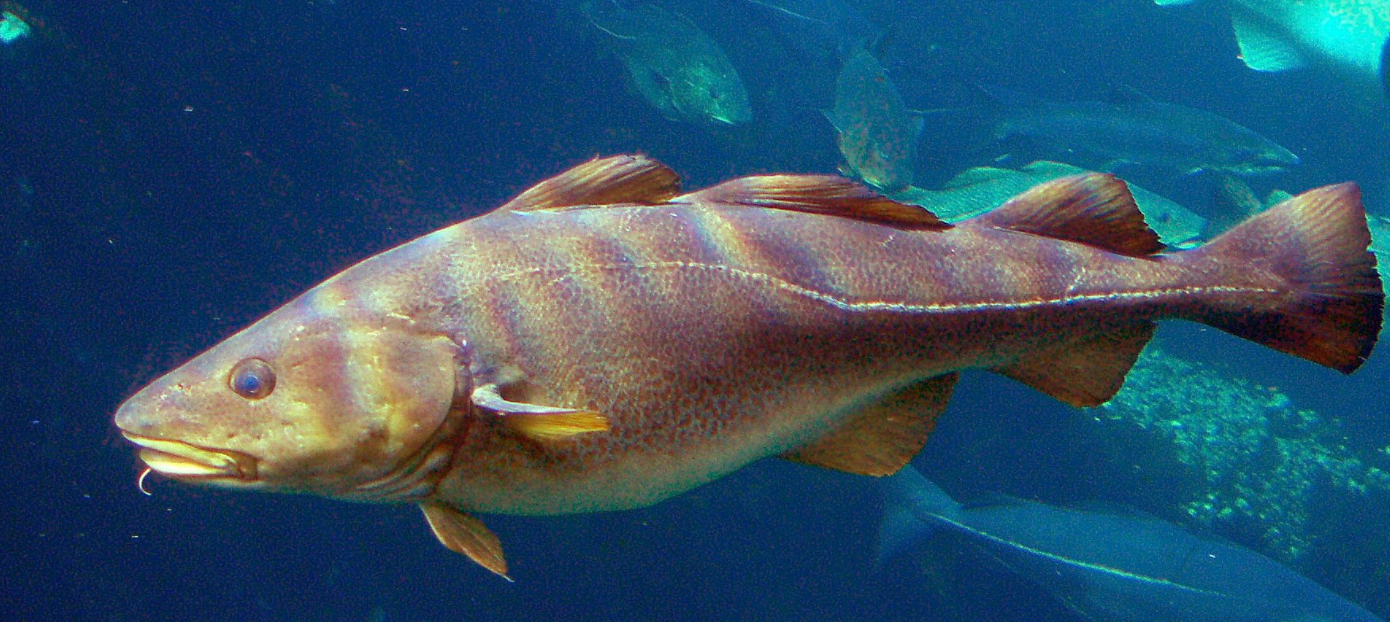
\includegraphics[width=0.5\textwidth,height=\textheight]{pictures/cod.png}
\caption{A cod fish, one of the top species captured by marine fisheries
(8)}
\end{figure}

\hypertarget{how-did-global-fishing-activity-change-during-the-covid-19-pandemic}{%
\subsection{How did global fishing activity change during the Covid-19
pandemic?}\label{how-did-global-fishing-activity-change-during-the-covid-19-pandemic}}

2020 is a year we will never forget. Covid-19 spread rapidly across the
globe and forced most of humanity into a state of quarantine. Covid-19
had clear devastating impacts on economies of all scales. Travel was
heavily limited, and even when crossing country borders was possible, it
was heavily monitored. However, the pandemic boosted some sectors of the
economy and increased demand for certain goods. How did Covid-19 impact
the fishing economy? Did fisheries respond to the pandemic by sending
fishermen and fisherwomen home to quarantine, or did some countries see
this as an opportunity to fish in the high seas more than ever before? I
could not find any literature that answers this question, which is
likely due to the fact that 2020 was less than a year ago, and any
formal studies on this topic might not have had time to be published.

Regulating fishing and other vessel activities across the globe is a
challenge in itself (4). Databases often have large gaps due to various
causes such as a lack of reliable data from automatic identification
systems and voluntary vessel registration by the owners of the vessels.
\href{https://globalfishingwatch.org/}{Global Fishing Watch} is an
organization that aims to revolutionize the way we monitor fishing
activity across the world using remote sensing techniques from
satellites combined with automatic identification systems. Global
Fishing Watch collects and visualizes global fishing data with the goal
of embracing ocean sustainability, transparency, and open-source
science. They keep track of vessels from all different countries,
including their movements, boat types, and time stamps for fishing and
docking at ports. Without such efforts to monitor, publicize, and
regulate ocean activity, our marine resources are at high risk of
depletion. On a global scale, we are fishing faster than fish stocks can
naturally replenish. This has severe economic impacts; according to the
World Bank Report, the ensuing depletion of marine fish stocks causes
economic losses of 50 billion US dollars annually (4). With modern data
science and applied statistics, we can better understand fishing
activity on a global scale and protect our planet's marine biodiversity.

As an aspiring wildlife biologist and data scientist, I'm interested in
applying statistical analysis to
\href{https://globalfishingwatch.org/datasets-and-code/}{Global Fishing
Watch data} to learn how different countries' fishing effort changed in
2020, relative to those countries' fishing trends in the years leading
up to 2020. In this dataset, fishing effort is defined by the amount of
hours spent fishing (3). I chose to use this dataset for my statistical
analysis because it is already relatively clean, I know the data is
relaible because Global Fishing Watch is a highly respected data
resource with highly accurate remotely sensed data that is combined with
locally collected automatic identification systems on shore, and I am
interested in working with Global Fishing Watch and spatial data in the
future. This data does not have spatial component since we treat
countries as a categorical variable, and the temporal variable is
limited to years. The only bias I believe might be present in this data
is that it is limited to boats that either voluntarily allow their
fishing hours to be tracked (such as through automatic identification
systems) as well as boats that have been detected remotely by satellite.

With Global Fishing Watch's expansive open-source data collection, we
can approach this question by grouping all vessels' fishing hours by
country, identifying a statistical trend up until 2019, and
extrapolating that trend into 2020. By comparing this 2020 prediction to
the actual fishing data available for 2020, we can glean how Covid-19
skewed large-scale fishing efforts. I chose this analysis approach
because I am familiar with these processes (besides the for loop aspect)
through my graduate statisics course and I believe it will be the
simplest and most accurate way to derive a p-value that will reveal if
there is a statistically significant difference between each country's
actual mean fishing effort and their predicted mean fishing effort in
2020. Perhaps the global fishing economy sky-rocketed, plummeted into
near nonexistence, or remained unscathed by the pandemic. Quantitative
analysis will help provide some insight.

Global Fishing Watch offers an
\href{https://globalfishingwatch.org/map/?latitude=19\&longitude=-30\&zoom=1.5\&start=2021-08-26T23\%3A00\%3A00.000Z\&end=2021-11-27T00\%3A00\%3A00.000Z}{interactive
map} that displays fishing activity across the globe through a heat map.
This visualization has the potential to inspire data scientists, fish
enthusiasts, environmental justice advocates, pandemic researchers, and
everyone in between to examine fishing activity during a time period of
interest.

\begin{figure}
\centering
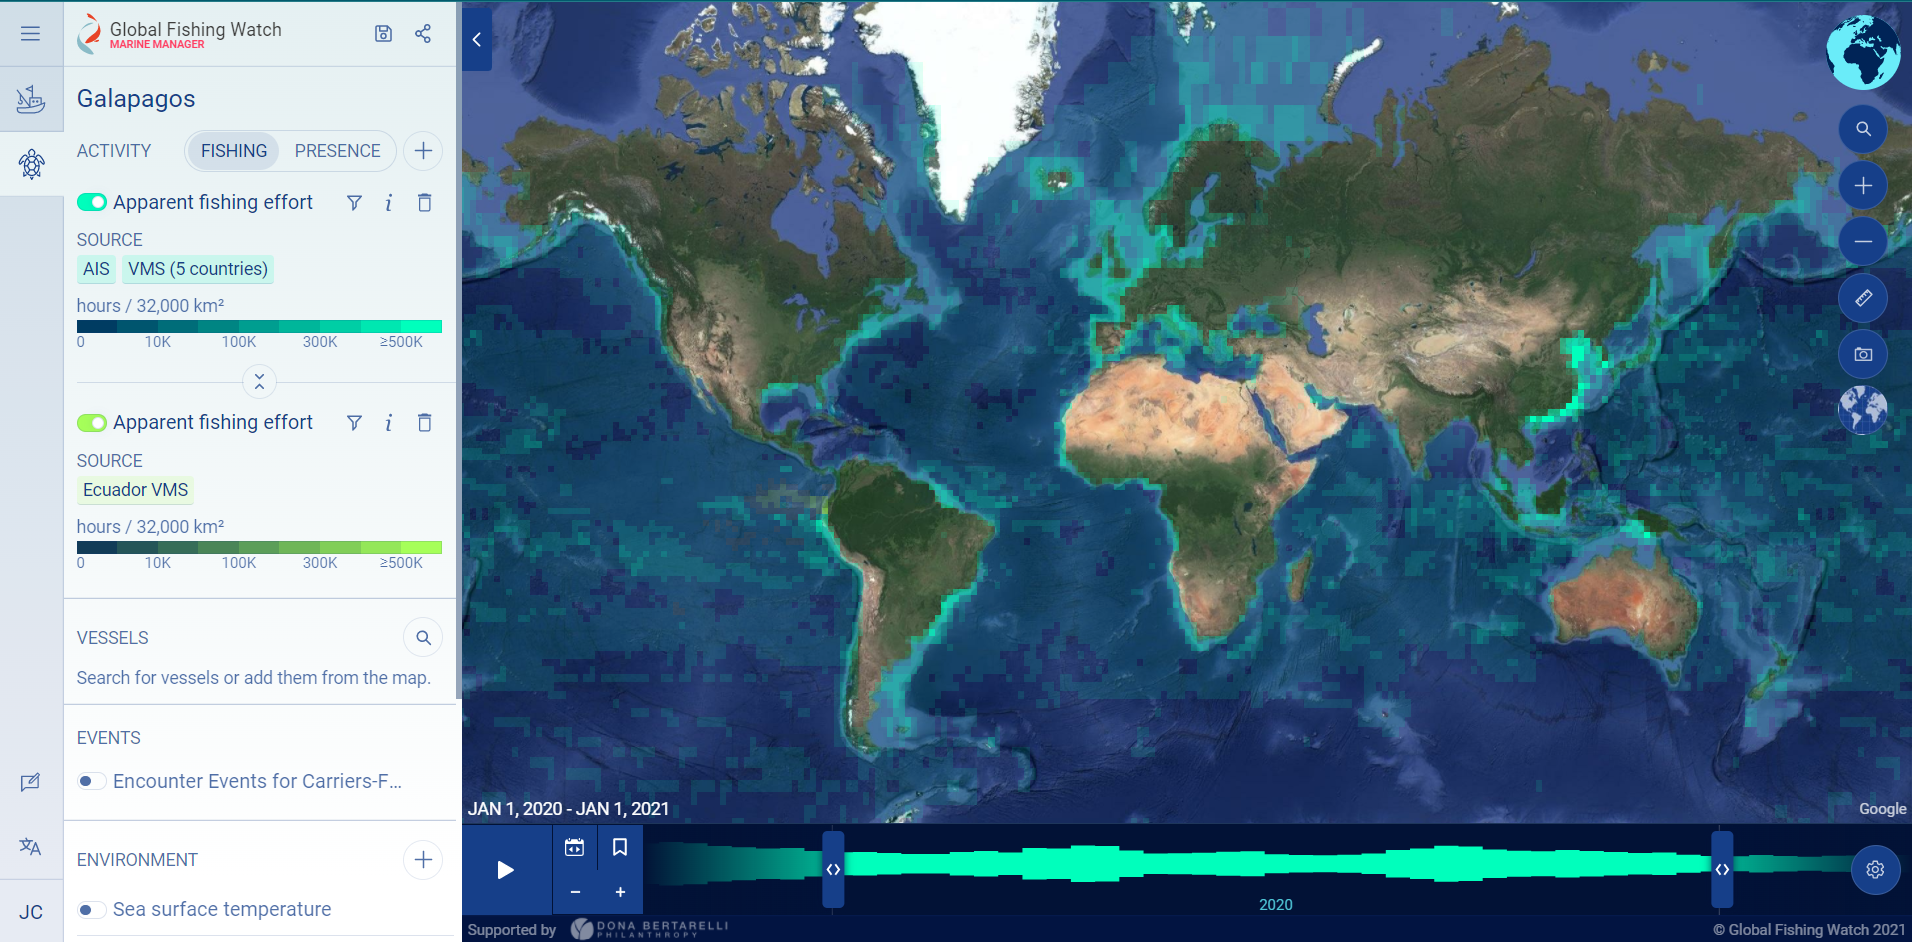
\includegraphics[width=0.7\textwidth,height=\textheight]{pictures/fishing_gfw_map_2020.png}
\caption{Global fishing activity from January 1, 2020 through January 1,
2021}
\end{figure}

Global Fishing Watch and their partners also provide an
\href{https://globalfishingwatch.org/carrier-portal/?latitude=12.7069821\&longitude=19.1776829\&zoom=1.1903704\&layer\%5B0\%5D=encounter\&layer\%5B1\%5D=cp_rfmo\&layer\%5B2\%5D=cp_next_port\&dataset=carriers:v20211001\&tab=flags}{interactive
map} that allows users to interact with vessels across the globe, filter
by country, and overlay port locations on coastlines.

\begin{Shaded}
\begin{Highlighting}[]
\CommentTok{\# the tidyverse includes my go{-}to set of functions for data cleaning and wrangling}
\FunctionTok{library}\NormalTok{(tidyverse)}
\end{Highlighting}
\end{Shaded}

\begin{verbatim}
## -- Attaching packages --------------------------------------- tidyverse 1.3.1 --
\end{verbatim}

\begin{verbatim}
## v ggplot2 3.3.5     v purrr   0.3.4
## v tibble  3.1.6     v dplyr   1.0.7
## v tidyr   1.1.4     v stringr 1.4.0
## v readr   2.1.1     v forcats 0.5.1
\end{verbatim}

\begin{verbatim}
## -- Conflicts ------------------------------------------ tidyverse_conflicts() --
## x dplyr::filter() masks stats::filter()
## x dplyr::lag()    masks stats::lag()
\end{verbatim}

\begin{Shaded}
\begin{Highlighting}[]
\CommentTok{\# lubridate helps us manage time stamps and annual trends}
\FunctionTok{library}\NormalTok{(lubridate)}
\end{Highlighting}
\end{Shaded}

\begin{verbatim}
## 
## Attaching package: 'lubridate'
\end{verbatim}

\begin{verbatim}
## The following objects are masked from 'package:base':
## 
##     date, intersect, setdiff, union
\end{verbatim}

\begin{Shaded}
\begin{Highlighting}[]
\CommentTok{\# gt helps make beautiful tables to summarize our data}
\FunctionTok{library}\NormalTok{(gt)}
\FunctionTok{library}\NormalTok{(broom)}
\FunctionTok{library}\NormalTok{(here)}
\end{Highlighting}
\end{Shaded}

\begin{verbatim}
## here() starts at /Users/juliet/Documents/MEDS/Fall_Quarter/EDS222_Statistics/final_project/fishing_effort
\end{verbatim}

\begin{Shaded}
\begin{Highlighting}[]
\NormalTok{data }\OtherTok{=} \FunctionTok{read\_csv}\NormalTok{(}\FunctionTok{file.path}\NormalTok{(}\StringTok{\textquotesingle{}data\textquotesingle{}}\NormalTok{, }\StringTok{\textquotesingle{}fishing{-}vessels{-}v2.csv\textquotesingle{}}\NormalTok{))}
\end{Highlighting}
\end{Shaded}

\begin{verbatim}
## Rows: 114191 Columns: 28
\end{verbatim}

\begin{verbatim}
## -- Column specification --------------------------------------------------------
## Delimiter: ","
## chr  (7): flag_ais, flag_registry, flag_gfw, vessel_class_inferred, vessel_c...
## dbl (20): mmsi, vessel_class_inferred_score, length_m_inferred, length_m_reg...
## lgl  (1): self_reported_fishing_vessel
\end{verbatim}

\begin{verbatim}
## 
## i Use `spec()` to retrieve the full column specification for this data.
## i Specify the column types or set `show_col_types = FALSE` to quiet this message.
\end{verbatim}

\hypertarget{data-cleaning-and-wrangling}{%
\subsubsection{Data Cleaning and
Wrangling}\label{data-cleaning-and-wrangling}}

Global Fishing Watch's data includes fishing effort and vessel
information from 124 countries over the years 2012-2020. First, we
select our variables of interest, group by country, and take the fishing
effort means per year (3).

\begin{Shaded}
\begin{Highlighting}[]
\CommentTok{\# clean the data, selecting only relevant column of fishing hours and taking the means by year for each country}

\NormalTok{effort\_trends }\OtherTok{\textless{}{-}}\NormalTok{ data }\SpecialCharTok{\%\textgreater{}\%} 
  \FunctionTok{select}\NormalTok{(flag\_gfw, }
\NormalTok{         fishing\_hours\_2012,}
\NormalTok{         fishing\_hours\_2013,}
\NormalTok{         fishing\_hours\_2014,}
\NormalTok{         fishing\_hours\_2015,}
\NormalTok{         fishing\_hours\_2016,}
\NormalTok{         fishing\_hours\_2017,}
\NormalTok{         fishing\_hours\_2018,}
\NormalTok{         fishing\_hours\_2019,}
\NormalTok{         fishing\_hours\_2020) }\SpecialCharTok{\%\textgreater{}\%} 
  \FunctionTok{group\_by}\NormalTok{(flag\_gfw) }\SpecialCharTok{\%\textgreater{}\%} 
  \FunctionTok{summarize}\NormalTok{(}\StringTok{"2012"} \OtherTok{=} \FunctionTok{mean}\NormalTok{(fishing\_hours\_2012, }\AttributeTok{na.rm =} \ConstantTok{TRUE}\NormalTok{),}
            \StringTok{"2013"} \OtherTok{=} \FunctionTok{mean}\NormalTok{(fishing\_hours\_2013, }\AttributeTok{na.rm =} \ConstantTok{TRUE}\NormalTok{),}
            \StringTok{"2014"} \OtherTok{=} \FunctionTok{mean}\NormalTok{(fishing\_hours\_2014, }\AttributeTok{na.rm =} \ConstantTok{TRUE}\NormalTok{),}
            \StringTok{"2015"} \OtherTok{=} \FunctionTok{mean}\NormalTok{(fishing\_hours\_2015, }\AttributeTok{na.rm =} \ConstantTok{TRUE}\NormalTok{),}
            \StringTok{"2016"} \OtherTok{=} \FunctionTok{mean}\NormalTok{(fishing\_hours\_2016, }\AttributeTok{na.rm =} \ConstantTok{TRUE}\NormalTok{),}
            \StringTok{"2017"} \OtherTok{=} \FunctionTok{mean}\NormalTok{(fishing\_hours\_2017, }\AttributeTok{na.rm =} \ConstantTok{TRUE}\NormalTok{),}
            \StringTok{"2018"} \OtherTok{=} \FunctionTok{mean}\NormalTok{(fishing\_hours\_2018, }\AttributeTok{na.rm =} \ConstantTok{TRUE}\NormalTok{),}
            \StringTok{"2019"} \OtherTok{=} \FunctionTok{mean}\NormalTok{(fishing\_hours\_2019, }\AttributeTok{na.rm =} \ConstantTok{TRUE}\NormalTok{),}
            \StringTok{"2020"} \OtherTok{=} \FunctionTok{mean}\NormalTok{(fishing\_hours\_2020, }\AttributeTok{na.rm =} \ConstantTok{TRUE}\NormalTok{))}
\end{Highlighting}
\end{Shaded}

Our goal is to run a linear regression on each country's fishing effort
over multiple years, but many countries have \texttt{NA} data for
certain years. Considering that we have data available for 2012-2020,
which years should we choose? We want to select a chunk of continuous
years leading up to 2020 with minimal data gaps. We want to minimize the
amount of \texttt{NA} values because we will drop all rows with
\texttt{NA} values, and we want to maintain the maximum amount of rows
(which represent vessels) and countries as possible. In order to choose
the start year for the time period that we will feed into the linear
regression, we'll take a look at the amount of \texttt{NA} values in the
years leading up to 2020. It turns out that 2017 has the least amount of
\texttt{NA} values, so we will use that year to start our 3-year data
period to feed to the linear regression. Next, we convert the data into
\textbf{Tidy} format and remove \texttt{NA} values so we can run a time
series linear regression analysis.

\begin{Shaded}
\begin{Highlighting}[]
\CommentTok{\# only need to look at 2012 {-} 2017 rather than 2012 {-} 2019 because we want a few years of data to plug into the linear regression}
\FunctionTok{sum}\NormalTok{(}\FunctionTok{is.na}\NormalTok{(effort\_trends}\SpecialCharTok{$}\StringTok{"2012"}\NormalTok{))}
\end{Highlighting}
\end{Shaded}

\begin{verbatim}
## [1] 83
\end{verbatim}

\begin{Shaded}
\begin{Highlighting}[]
\FunctionTok{sum}\NormalTok{(}\FunctionTok{is.na}\NormalTok{(effort\_trends}\SpecialCharTok{$}\StringTok{"2013"}\NormalTok{))}
\end{Highlighting}
\end{Shaded}

\begin{verbatim}
## [1] 71
\end{verbatim}

\begin{Shaded}
\begin{Highlighting}[]
\FunctionTok{sum}\NormalTok{(}\FunctionTok{is.na}\NormalTok{(effort\_trends}\SpecialCharTok{$}\StringTok{"2014"}\NormalTok{))}
\end{Highlighting}
\end{Shaded}

\begin{verbatim}
## [1] 60
\end{verbatim}

\begin{Shaded}
\begin{Highlighting}[]
\FunctionTok{sum}\NormalTok{(}\FunctionTok{is.na}\NormalTok{(effort\_trends}\SpecialCharTok{$}\StringTok{"2015"}\NormalTok{))}
\end{Highlighting}
\end{Shaded}

\begin{verbatim}
## [1] 52
\end{verbatim}

\begin{Shaded}
\begin{Highlighting}[]
\FunctionTok{sum}\NormalTok{(}\FunctionTok{is.na}\NormalTok{(effort\_trends}\SpecialCharTok{$}\StringTok{"2016"}\NormalTok{))}
\end{Highlighting}
\end{Shaded}

\begin{verbatim}
## [1] 42
\end{verbatim}

\begin{Shaded}
\begin{Highlighting}[]
\FunctionTok{sum}\NormalTok{(}\FunctionTok{is.na}\NormalTok{(effort\_trends}\SpecialCharTok{$}\StringTok{"2017"}\NormalTok{))}
\end{Highlighting}
\end{Shaded}

\begin{verbatim}
## [1] 37
\end{verbatim}

\begin{Shaded}
\begin{Highlighting}[]
\CommentTok{\# change it to tidy format using pivot\_longer()}
\CommentTok{\# remove all NA values, and take out the year 2020 because we want to compare what we would EXPECT in 2020 based on what we saw in 2017{-}2019}

\NormalTok{effort\_trends\_tidy\_no\_na }\OtherTok{=}\NormalTok{ effort\_trends }\SpecialCharTok{\%\textgreater{}\%}
  \FunctionTok{select}\NormalTok{(flag\_gfw, }\StringTok{"2017"}\SpecialCharTok{:}\StringTok{"2019"}\NormalTok{) }\SpecialCharTok{\%\textgreater{}\%} 
  \FunctionTok{pivot\_longer}\NormalTok{(}\AttributeTok{cols =}\NormalTok{ (}\StringTok{"2017"}\SpecialCharTok{:}\StringTok{"2019"}\NormalTok{),}
               \AttributeTok{names\_to =} \StringTok{"year"}\NormalTok{,}
               \AttributeTok{values\_to =} \StringTok{"mean\_effort"}\NormalTok{) }\SpecialCharTok{\%\textgreater{}\%} 
  \FunctionTok{filter}\NormalTok{(}\SpecialCharTok{!}\FunctionTok{is.na}\NormalTok{(mean\_effort),}
         \SpecialCharTok{!}\FunctionTok{is.na}\NormalTok{(flag\_gfw))}
\end{Highlighting}
\end{Shaded}

Our dates are in years, and currently their class is \texttt{character}
in the original dataset. We need these years in \texttt{date} format in
order to run a linear regression over time. We will convert these years
and remove all countries that only have data for 1 or 2 years, because
we need multiple years of data to feed into the regression and we want
each country to have equal amounts of data and start in the year 2017.

\begin{Shaded}
\begin{Highlighting}[]
\CommentTok{\# define day as Jan 1 so that when we convert the year to a date we get the first of the year so the plot looks better later on! Otherwise, R will paste TODAY\textquotesingle{}S date at the end of each year, which will skew the x axis when we plot later}

\NormalTok{month\_day }\OtherTok{\textless{}{-}} \StringTok{"{-}01{-}01"}
\NormalTok{effort\_trends\_tidy\_no\_na\_date }\OtherTok{\textless{}{-}}\NormalTok{ effort\_trends\_tidy\_no\_na }\SpecialCharTok{\%\textgreater{}\%} 
  \FunctionTok{mutate}\NormalTok{(}\AttributeTok{year =} \FunctionTok{paste0}\NormalTok{(year, month\_day))}

\CommentTok{\# remove those countries from the dataframe}
\NormalTok{countries\_clean }\OtherTok{\textless{}{-}}\NormalTok{ effort\_trends\_tidy\_no\_na\_date }\SpecialCharTok{\%\textgreater{}\%} 
  \FunctionTok{group\_by}\NormalTok{(flag\_gfw) }\SpecialCharTok{\%\textgreater{}\%}
  \FunctionTok{filter}\NormalTok{(}\FunctionTok{n}\NormalTok{()}\SpecialCharTok{\textgreater{}}\DecValTok{2}\NormalTok{) }\SpecialCharTok{\%\textgreater{}\%} 
  \FunctionTok{mutate}\NormalTok{(}\AttributeTok{year =} \FunctionTok{as.Date}\NormalTok{(year, }\AttributeTok{format =} \StringTok{"\%Y{-}\%m{-}\%d"}\NormalTok{))}
\end{Highlighting}
\end{Shaded}

\hypertarget{linear-regression}{%
\subsubsection{Linear Regression}\label{linear-regression}}

Now that the data is sufficiently clean and our years are of class
\texttt{date}, we can run a time series linear regression on every
country's fishing effort from 2017-2019 and use the output coefficients
to glean which direction each country is trending, meaning if the
country is fishing more or less over time. We can do this with the
\texttt{do()} function, grouping by country. We can set the function to
output all the model coefficients as a list. Then we can feed this
output into a for loop! We can plug in each country's fishing effort
intercept and slope coefficients into a linear equation to predict the
fishing effort in 2020 based on that country's historical trend.
Subsequently, we can combine the predicted 2020 fishing effort data with
the actual 2020 fishing effort data into a single dataframe to compare
by country. We can make a new column that takes the difference of the
actual and predicted values, and then add a column that explicitly
states whether that country increased or decreased their fishing effort
in 2020 relative to their trend leading up to 2020.

\begin{Shaded}
\begin{Highlighting}[]
\CommentTok{\# countries\_clean \%\textgreater{}\% }
\CommentTok{\#   group\_by(flag\_gfw) \%\textgreater{}\% }
\CommentTok{\#   do(data.frame(., as.list(coef(lm(mean\_effort\textasciitilde{}year, .)))))}

\CommentTok{\# try to adjust the code that worked earlier to be like this code}
\NormalTok{models }\OtherTok{\textless{}{-}} \FunctionTok{sapply}\NormalTok{(}\FunctionTok{unique}\NormalTok{(}\FunctionTok{as.character}\NormalTok{(countries\_clean}\SpecialCharTok{$}\NormalTok{flag\_gfw)),}
                 \ControlFlowTok{function}\NormalTok{(country)}\FunctionTok{as.numeric}\NormalTok{(}\FunctionTok{coef}\NormalTok{(}\FunctionTok{lm}\NormalTok{(mean\_effort}\SpecialCharTok{\textasciitilde{}}\NormalTok{year, countries\_clean, }\AttributeTok{subset =}\NormalTok{ (flag\_gfw }\SpecialCharTok{==}\NormalTok{ country)))),}
                 \AttributeTok{simplify =} \ConstantTok{FALSE}\NormalTok{, }\AttributeTok{USE.NAMES =} \ConstantTok{TRUE}\NormalTok{)}
\CommentTok{\# \#models[[4]]}
\NormalTok{models}
\end{Highlighting}
\end{Shaded}

\begin{verbatim}
## $AFG
## [1] -714.80545358    0.05827854
## 
## $AGO
## [1] 21327.016810    -1.067632
## 
## $ALB
## [1] -1.596739e+04  9.645507e-01
## 
## $ARG
## [1] 3063.66187503   -0.07661104
## 
## $AUS
## [1] 3921.2952177   -0.1580011
## 
## $BEL
## [1] 127.9329249   0.1010738
## 
## $BGR
## [1] -5261.5617204     0.3304856
## 
## $BHR
## [1] 1517.2470462   -0.0673782
## 
## $BLZ
## [1] -4622.7249189     0.3497073
## 
## $BRA
## [1] -8515.3602549     0.5793368
## 
## $CAN
## [1] -981.83548906    0.08690468
## 
## $CHL
## [1] -264.74111524    0.08088757
## 
## $CHN
## [1] 29.62881691  0.02518987
## 
## $CIV
## [1] 2.547609e+03 1.856164e-02
## 
## $CMR
## [1] -9204.1040274     0.6303356
## 
## $COK
## [1] -48314.270956      2.911865
## 
## $COL
## [1] 8752.8165464   -0.4073048
## 
## $CPV
## [1] -6002.9961766     0.3631073
## 
## $CUW
## [1] 1284.01742283   -0.01806301
## 
## $CYP
## [1] 2076.29528456   -0.05079806
## 
## $DEU
## [1] 2095.5655134   -0.0680371
## 
## $DNK
## [1] 2196.97223216   -0.06059565
## 
## $DZA
## [1] 1121.73616797   -0.05609932
## 
## $ECU
## [1] -659.64954106    0.06893002
## 
## $ESP
## [1] -615.0444411    0.1107815
## 
## $EST
## [1] -622.5661735    0.1257922
## 
## $FIN
## [1] 2440.2490638   -0.0688222
## 
## $FJI
## [1] -213.6159167    0.2422723
## 
## $FLK
## [1] 11355.1833654    -0.5032467
## 
## $FRA
## [1] 5379.6843296   -0.2144988
## 
## $FRO
## [1] 19895.1638899    -0.9866422
## 
## $FSM
## [1] 12434.0689049    -0.5690816
## 
## $GBR
## [1] 360.0061351   0.0469582
## 
## $GEO
## [1] -9041.968690     0.532414
## 
## $GHA
## [1] -7880.47333     0.54624
## 
## $GIN
## [1] -1805.7444027     0.3037836
## 
## $GNB
## [1] 4633.5533382   -0.1397766
## 
## $GNQ
## [1] -6393.9150030     0.3723151
## 
## $GRC
## [1] 2084.47738320   -0.06161967
## 
## $GRL
## [1] 793.28932701   0.07808875
## 
## $GTM
## [1] 10013.1072892    -0.5200982
## 
## $HKG
## [1] 1630.8647169   -0.0726153
## 
## $HND
## [1] 342.944913242  -0.001520548
## 
## $HRV
## [1] 2463.25447610   -0.06901769
## 
## $IDN
## [1] -3226.9648492     0.2321137
## 
## $IND
## [1] 2454.6660117   -0.1121845
## 
## $IRL
## [1] 3037.26045245   -0.09702787
## 
## $IRN
## [1] 11384.0975985    -0.6051754
## 
## $ISL
## [1] -696.4228684    0.0735052
## 
## $ISR
## [1] -1617.9595605     0.1902396
## 
## $ITA
## [1] 1911.64669779   -0.02387959
## 
## $JPN
## [1] 8393.6803979   -0.4077772
## 
## $KEN
## [1] -36602.435559      2.152315
## 
## $KIR
## [1] 23216.297257    -1.259444
## 
## $KNA
## [1] -1532.709747     0.119516
## 
## $KOR
## [1] 2919.7421770   -0.1158657
## 
## $LBR
## [1] 6871.3841598   -0.1985411
## 
## $LBY
## [1] -4532.2914547     0.2716906
## 
## $LKA
## [1] -21325.294911      1.280157
## 
## $LTU
## [1] 2544.26587835   -0.08547912
## 
## $LVA
## [1] 4843.2114930   -0.2305974
## 
## $MAR
## [1] -6841.5041176     0.5868073
## 
## $MEX
## [1]  1.552772e+03 -6.824276e-03
## 
## $MHL
## [1] 6533.6593738   -0.2601237
## 
## $MLT
## [1] 4260.735175   -0.194258
## 
## $MNE
## [1] -1.108627e+04  6.660597e-01
## 
## $MOZ
## [1] 33643.495361    -1.748183
## 
## $MRT
## [1] 5336.9208555   -0.1806169
## 
## $MUS
## [1] 5971.0531495   -0.2555744
## 
## $MYS
## [1] 889.650985154  -0.002102247
## 
## $NAM
## [1] -3076.1052970     0.3168376
## 
## $NCL
## [1] 19092.5063842    -0.9483393
## 
## $NGA
## [1] -30917.499542      1.848851
## 
## $NIC
## [1] 13662.5800715    -0.7277374
## 
## $NLD
## [1] 6933.3796998   -0.3124013
## 
## $NOR
## [1] 1082.55165308   -0.03431382
## 
## $NRU
## [1] 24875.944707    -1.362645
## 
## $NZL
## [1] 5128.6133775   -0.1680471
## 
## $PAN
## [1] -1.258200e+04  7.763052e-01
## 
## $PER
## [1] -1.021280e+03  8.643745e-02
## 
## $PHL
## [1] 6055.9519876   -0.3043986
## 
## $PNG
## [1] 7548.3639607   -0.3446986
## 
## $POL
## [1] 3380.0020459   -0.1516196
## 
## $PRT
## [1] 6398.6117848   -0.2797066
## 
## $PYF
## [1] 16571.9405810    -0.8206569
## 
## $QAT
## [1] -2010.634928     0.152422
## 
## $REU
## [1] -4000.3655880     0.2383863
## 
## $ROU
## [1] 8358.5565644   -0.4437137
## 
## $RUS
## [1] 9123.9407520   -0.3715655
## 
## $SAU
## [1] 1434.55678440   -0.05690642
## 
## $SEN
## [1] 2.225963e+03 3.182057e-02
## 
## $SGP
## [1] -5544.8346423     0.3401461
## 
## $SHN
## [1] -1.597960e+04  9.955342e-01
## 
## $SLB
## [1] -1633.3677128     0.1533233
## 
## $SLV
## [1] 4789.3423440   -0.2292694
## 
## $SPM
## [1] -5482.2204125     0.3378584
## 
## $SVN
## [1] 7471.6207196   -0.3859743
## 
## $SWE
## [1] -796.56950659    0.09087399
## 
## $SYC
## [1] 11037.8085236    -0.4368539
## 
## $TCA
## [1] 3571.8647945   -0.1512329
## 
## $THA
## [1] -6075.1626421     0.3734093
## 
## $TUN
## [1] -822.76561686    0.07797797
## 
## $TUR
## [1] 178.95089336   0.01674968
## 
## $TUV
## [1] 21420.455737    -1.181913
## 
## $TWN
## [1] -2083.134045     0.220274
## 
## $UKR
## [1] 11124.2167774    -0.5461355
## 
## $UNK
## [1] 76.41393304  0.01577577
## 
## $URY
## [1] 3842.7719406   -0.0716254
## 
## $USA
## [1] 984.33283681  -0.01264758
## 
## $VCT
## [1] -43066.969024      2.617025
## 
## $VEN
## [1] 3644.7952118   -0.1653996
## 
## $VNM
## [1] -5776.8390125     0.3437493
## 
## $VUT
## [1] 12868.0275701    -0.4975337
## 
## $ZAF
## [1] 693.32480379   0.04447054
\end{verbatim}

\begin{Shaded}
\begin{Highlighting}[]
\NormalTok{countries\_in\_models }\OtherTok{\textless{}{-}} \FunctionTok{unique}\NormalTok{(}\FunctionTok{as.character}\NormalTok{(countries\_clean}\SpecialCharTok{$}\NormalTok{flag\_gfw))}
\NormalTok{countries\_in\_models}
\end{Highlighting}
\end{Shaded}

\begin{verbatim}
##   [1] "AFG" "AGO" "ALB" "ARG" "AUS" "BEL" "BGR" "BHR" "BLZ" "BRA" "CAN" "CHL"
##  [13] "CHN" "CIV" "CMR" "COK" "COL" "CPV" "CUW" "CYP" "DEU" "DNK" "DZA" "ECU"
##  [25] "ESP" "EST" "FIN" "FJI" "FLK" "FRA" "FRO" "FSM" "GBR" "GEO" "GHA" "GIN"
##  [37] "GNB" "GNQ" "GRC" "GRL" "GTM" "HKG" "HND" "HRV" "IDN" "IND" "IRL" "IRN"
##  [49] "ISL" "ISR" "ITA" "JPN" "KEN" "KIR" "KNA" "KOR" "LBR" "LBY" "LKA" "LTU"
##  [61] "LVA" "MAR" "MEX" "MHL" "MLT" "MNE" "MOZ" "MRT" "MUS" "MYS" "NAM" "NCL"
##  [73] "NGA" "NIC" "NLD" "NOR" "NRU" "NZL" "PAN" "PER" "PHL" "PNG" "POL" "PRT"
##  [85] "PYF" "QAT" "REU" "ROU" "RUS" "SAU" "SEN" "SGP" "SHN" "SLB" "SLV" "SPM"
##  [97] "SVN" "SWE" "SYC" "TCA" "THA" "TUN" "TUR" "TUV" "TWN" "UKR" "UNK" "URY"
## [109] "USA" "VCT" "VEN" "VNM" "VUT" "ZAF"
\end{verbatim}

\begin{Shaded}
\begin{Highlighting}[]
\CommentTok{\# }
\NormalTok{prediction\_data }\OtherTok{=} \ConstantTok{NULL}\NormalTok{;}
\ControlFlowTok{for}\NormalTok{ (i }\ControlFlowTok{in} \DecValTok{1}\SpecialCharTok{:}\FunctionTok{length}\NormalTok{(models)) \{}
\NormalTok{  predicted\_effort\_2020 }\OtherTok{\textless{}{-}}\NormalTok{ models[[i]][}\DecValTok{1}\NormalTok{] }\SpecialCharTok{+}\NormalTok{ models[[i]][}\DecValTok{2}\NormalTok{]}\SpecialCharTok{*}\DecValTok{3}
\NormalTok{  prediction\_data }\OtherTok{\textless{}{-}} \FunctionTok{rbind}\NormalTok{(prediction\_data, predicted\_effort\_2020)}
  \FunctionTok{print}\NormalTok{(}\FunctionTok{paste0}\NormalTok{(}\StringTok{"In 2020, the predicted fishing hours is "}\NormalTok{, predicted\_effort\_2020))}
\NormalTok{\}}
\end{Highlighting}
\end{Shaded}

\begin{verbatim}
## [1] "In 2020, the predicted fishing hours is -714.630617960425"
## [1] "In 2020, the predicted fishing hours is 21323.8139148635"
## [1] "In 2020, the predicted fishing hours is -15964.5013093548"
## [1] "In 2020, the predicted fishing hours is 3063.43204190972"
## [1] "In 2020, the predicted fishing hours is 3920.82121431707"
## [1] "In 2020, the predicted fishing hours is 128.23614639422"
## [1] "In 2020, the predicted fishing hours is -5260.57026370865"
## [1] "In 2020, the predicted fishing hours is 1517.044911641"
## [1] "In 2020, the predicted fishing hours is -4621.67579709532"
## [1] "In 2020, the predicted fishing hours is -8513.62224455465"
## [1] "In 2020, the predicted fishing hours is -981.574775032544"
## [1] "In 2020, the predicted fishing hours is -264.498452521068"
## [1] "In 2020, the predicted fishing hours is 29.7043865127327"
## [1] "In 2020, the predicted fishing hours is 2547.66461187216"
## [1] "In 2020, the predicted fishing hours is -9202.21302054795"
## [1] "In 2020, the predicted fishing hours is -48305.5353603756"
## [1] "In 2020, the predicted fishing hours is 8751.59463203964"
## [1] "In 2020, the predicted fishing hours is -6001.90685464233"
## [1] "In 2020, the predicted fishing hours is 1283.96323378996"
## [1] "In 2020, the predicted fishing hours is 2076.14289036648"
## [1] "In 2020, the predicted fishing hours is 2095.36140210988"
## [1] "In 2020, the predicted fishing hours is 2196.79044520795"
## [1] "In 2020, the predicted fishing hours is 1121.5678700261"
## [1] "In 2020, the predicted fishing hours is -659.442750983932"
## [1] "In 2020, the predicted fishing hours is -614.712096534242"
## [1] "In 2020, the predicted fishing hours is -622.188796803659"
## [1] "In 2020, the predicted fishing hours is 2440.04259718047"
## [1] "In 2020, the predicted fishing hours is -212.889099692058"
## [1] "In 2020, the predicted fishing hours is 11353.6736253739"
## [1] "In 2020, the predicted fishing hours is 5379.04083328041"
## [1] "In 2020, the predicted fishing hours is 19892.2039631442"
## [1] "In 2020, the predicted fishing hours is 12432.3616601726"
## [1] "In 2020, the predicted fishing hours is 360.147009683571"
## [1] "In 2020, the predicted fishing hours is -9040.37144824968"
## [1] "In 2020, the predicted fishing hours is -7878.83460609789"
## [1] "In 2020, the predicted fishing hours is -1804.83305205488"
## [1] "In 2020, the predicted fishing hours is 4633.1340082446"
## [1] "In 2020, the predicted fishing hours is -6392.7980578387"
## [1] "In 2020, the predicted fishing hours is 2084.29252418284"
## [1] "In 2020, the predicted fishing hours is 793.523593267236"
## [1] "In 2020, the predicted fishing hours is 10011.5469946728"
## [1] "In 2020, the predicted fishing hours is 1630.64687100459"
## [1] "In 2020, the predicted fishing hours is 342.940351598192"
## [1] "In 2020, the predicted fishing hours is 2463.04742303282"
## [1] "In 2020, the predicted fishing hours is -3226.26850813617"
## [1] "In 2020, the predicted fishing hours is 2454.32945813705"
## [1] "In 2020, the predicted fishing hours is 3036.96936884982"
## [1] "In 2020, the predicted fishing hours is 11382.2820722007"
## [1] "In 2020, the predicted fishing hours is -696.202352791085"
## [1] "In 2020, the predicted fishing hours is -1617.38884173934"
## [1] "In 2020, the predicted fishing hours is 1911.57505901916"
## [1] "In 2020, the predicted fishing hours is 8392.45706642112"
## [1] "In 2020, the predicted fishing hours is -36595.9786133945"
## [1] "In 2020, the predicted fishing hours is 23212.5189251469"
## [1] "In 2020, the predicted fishing hours is -1532.3511993912"
## [1] "In 2020, the predicted fishing hours is 2919.39457993244"
## [1] "In 2020, the predicted fishing hours is 6870.78853652997"
## [1] "In 2020, the predicted fishing hours is -4531.47638305432"
## [1] "In 2020, the predicted fishing hours is -21321.4544392909"
## [1] "In 2020, the predicted fishing hours is 2544.00944098046"
## [1] "In 2020, the predicted fishing hours is 4842.51970070318"
## [1] "In 2020, the predicted fishing hours is -6839.74369586345"
## [1] "In 2020, the predicted fishing hours is 1552.75177853496"
## [1] "In 2020, the predicted fishing hours is 6532.87900258756"
## [1] "In 2020, the predicted fishing hours is 4260.15240128292"
## [1] "In 2020, the predicted fishing hours is -11084.2763337188"
## [1] "In 2020, the predicted fishing hours is 33638.2508125572"
## [1] "In 2020, the predicted fishing hours is 5336.37900472927"
## [1] "In 2020, the predicted fishing hours is 5970.28642638358"
## [1] "In 2020, the predicted fishing hours is 889.64467841351"
## [1] "In 2020, the predicted fishing hours is -3075.15478425483"
## [1] "In 2020, the predicted fishing hours is 19089.6613661812"
## [1] "In 2020, the predicted fishing hours is -30911.9529894978"
## [1] "In 2020, the predicted fishing hours is 13660.3968592086"
## [1] "In 2020, the predicted fishing hours is 6932.44249590471"
## [1] "In 2020, the predicted fishing hours is 1082.44871161888"
## [1] "In 2020, the predicted fishing hours is 24871.8567711822"
## [1] "In 2020, the predicted fishing hours is 5128.10923634413"
## [1] "In 2020, the predicted fishing hours is -12579.6721244088"
## [1] "In 2020, the predicted fishing hours is -1021.0202325802"
## [1] "In 2020, the predicted fishing hours is 6055.03879174114"
## [1] "In 2020, the predicted fishing hours is 7547.32986495483"
## [1] "In 2020, the predicted fishing hours is 3379.54718696408"
## [1] "In 2020, the predicted fishing hours is 6397.77266508881"
## [1] "In 2020, the predicted fishing hours is 16569.4786103501"
## [1] "In 2020, the predicted fishing hours is -2010.17766169026"
## [1] "In 2020, the predicted fishing hours is -3999.65042909331"
## [1] "In 2020, the predicted fishing hours is 8357.22542328771"
## [1] "In 2020, the predicted fishing hours is 9122.82605552599"
## [1] "In 2020, the predicted fishing hours is 1434.38606512835"
## [1] "In 2020, the predicted fishing hours is 2226.05861345844"
## [1] "In 2020, the predicted fishing hours is -5543.81420395741"
## [1] "In 2020, the predicted fishing hours is -15976.6181415525"
## [1] "In 2020, the predicted fishing hours is -1632.90774292241"
## [1] "In 2020, the predicted fishing hours is 4788.65453576867"
## [1] "In 2020, the predicted fishing hours is -5481.20683713852"
## [1] "In 2020, the predicted fishing hours is 7470.46279661342"
## [1] "In 2020, the predicted fishing hours is -796.296884629973"
## [1] "In 2020, the predicted fishing hours is 11036.4979619368"
## [1] "In 2020, the predicted fishing hours is 3571.41109589051"
## [1] "In 2020, the predicted fishing hours is -6074.04241411181"
## [1] "In 2020, the predicted fishing hours is -822.531682937372"
## [1] "In 2020, the predicted fishing hours is 179.001142417618"
## [1] "In 2020, the predicted fishing hours is 21416.9099969559"
## [1] "In 2020, the predicted fishing hours is -2082.47322266226"
## [1] "In 2020, the predicted fishing hours is 11122.5783709424"
## [1] "In 2020, the predicted fishing hours is 76.4612603436158"
## [1] "In 2020, the predicted fishing hours is 3842.55706445384"
## [1] "In 2020, the predicted fishing hours is 984.294894057463"
## [1] "In 2020, the predicted fishing hours is -43059.1179482498"
## [1] "In 2020, the predicted fishing hours is 3644.29901302408"
## [1] "In 2020, the predicted fishing hours is -5775.80776451778"
## [1] "In 2020, the predicted fishing hours is 12866.5349689352"
## [1] "In 2020, the predicted fishing hours is 693.458215405196"
\end{verbatim}

\begin{Shaded}
\begin{Highlighting}[]
\CommentTok{\# figure out which countries were used in the for loop so we can get the actual 2020 effort data for those countries only}
\NormalTok{countries\_clean\_unique }\OtherTok{\textless{}{-}}\NormalTok{ countries\_clean }\SpecialCharTok{\%\textgreater{}\%} 
  \FunctionTok{group\_by}\NormalTok{(flag\_gfw) }\SpecialCharTok{\%\textgreater{}\%}
  \FunctionTok{slice\_head}\NormalTok{(}\AttributeTok{n =} \DecValTok{1}\NormalTok{)}

\CommentTok{\# set these countries as a vector so we can subset the effort\_trends data to only include those countries}
\NormalTok{countries\_to\_compare }\OtherTok{\textless{}{-}} \FunctionTok{unique}\NormalTok{(countries\_clean\_unique}\SpecialCharTok{$}\NormalTok{flag\_gfw)}
\NormalTok{countries\_to\_compare}
\end{Highlighting}
\end{Shaded}

\begin{verbatim}
##   [1] "AFG" "AGO" "ALB" "ARG" "AUS" "BEL" "BGR" "BHR" "BLZ" "BRA" "CAN" "CHL"
##  [13] "CHN" "CIV" "CMR" "COK" "COL" "CPV" "CUW" "CYP" "DEU" "DNK" "DZA" "ECU"
##  [25] "ESP" "EST" "FIN" "FJI" "FLK" "FRA" "FRO" "FSM" "GBR" "GEO" "GHA" "GIN"
##  [37] "GNB" "GNQ" "GRC" "GRL" "GTM" "HKG" "HND" "HRV" "IDN" "IND" "IRL" "IRN"
##  [49] "ISL" "ISR" "ITA" "JPN" "KEN" "KIR" "KNA" "KOR" "LBR" "LBY" "LKA" "LTU"
##  [61] "LVA" "MAR" "MEX" "MHL" "MLT" "MNE" "MOZ" "MRT" "MUS" "MYS" "NAM" "NCL"
##  [73] "NGA" "NIC" "NLD" "NOR" "NRU" "NZL" "PAN" "PER" "PHL" "PNG" "POL" "PRT"
##  [85] "PYF" "QAT" "REU" "ROU" "RUS" "SAU" "SEN" "SGP" "SHN" "SLB" "SLV" "SPM"
##  [97] "SVN" "SWE" "SYC" "TCA" "THA" "TUN" "TUR" "TUV" "TWN" "UKR" "UNK" "URY"
## [109] "USA" "VCT" "VEN" "VNM" "VUT" "ZAF"
\end{verbatim}

\begin{Shaded}
\begin{Highlighting}[]
\CommentTok{\# ensure that there are the same number of rows (countries) in both datasets}
\FunctionTok{nrow}\NormalTok{(countries\_clean\_unique)}
\end{Highlighting}
\end{Shaded}

\begin{verbatim}
## [1] 114
\end{verbatim}

\begin{Shaded}
\begin{Highlighting}[]
\FunctionTok{nrow}\NormalTok{(prediction\_data)}
\end{Highlighting}
\end{Shaded}

\begin{verbatim}
## [1] 114
\end{verbatim}

\begin{Shaded}
\begin{Highlighting}[]
\CommentTok{\# set the effort trends data to only include those countries}
\NormalTok{comparison\_2020 }\OtherTok{\textless{}{-}}\NormalTok{ effort\_trends }\SpecialCharTok{\%\textgreater{}\%} 
  \FunctionTok{select}\NormalTok{(flag\_gfw, }\StringTok{"2020"}\NormalTok{) }\SpecialCharTok{\%\textgreater{}\%}
  \FunctionTok{rename}\NormalTok{(}\AttributeTok{actual\_2020 =} \StringTok{"2020"}\NormalTok{) }\SpecialCharTok{\%\textgreater{}\%} 
  \FunctionTok{filter}\NormalTok{(}\FunctionTok{str\_detect}\NormalTok{(flag\_gfw, }\FunctionTok{paste}\NormalTok{(countries\_to\_compare, }\AttributeTok{collapse=}\StringTok{"|"}\NormalTok{))) }\SpecialCharTok{\%\textgreater{}\%} 
  \FunctionTok{cbind}\NormalTok{(prediction\_data) }\SpecialCharTok{\%\textgreater{}\%} 
  \FunctionTok{rename}\NormalTok{(}\AttributeTok{prediction\_2020 =}\NormalTok{ prediction\_data) }\SpecialCharTok{\%\textgreater{}\%} 
  \FunctionTok{filter}\NormalTok{(actual\_2020 }\SpecialCharTok{!=} \StringTok{"NaN"}\NormalTok{)}
\CommentTok{\# I made sure to remove the NAN values from the countries that did not have actual data for 2020 AFTER I USED cbind() because I wanted to bind the actual 2020 data to the corresponding rows with the predicted data first or else the alignment would yield incorrect data}

\CommentTok{\# remove all negative values in the predicted column, the linear regression did not fit this data well}
\NormalTok{comparison\_2020\_pos }\OtherTok{\textless{}{-}}\NormalTok{ comparison\_2020 }\SpecialCharTok{\%\textgreater{}\%} 
  \FunctionTok{filter}\NormalTok{(prediction\_2020 }\SpecialCharTok{\textgreater{}=} \DecValTok{0}\NormalTok{)}

\CommentTok{\# take the difference between the actual and the predicted columns}
\NormalTok{comparison\_2020\_pos }\OtherTok{\textless{}{-}}\NormalTok{ comparison\_2020\_pos }\SpecialCharTok{\%\textgreater{}\%} 
  \FunctionTok{mutate}\NormalTok{(}\AttributeTok{difference\_a\_minus\_p =}\NormalTok{ actual\_2020 }\SpecialCharTok{{-}}\NormalTok{ prediction\_2020) }\SpecialCharTok{\%\textgreater{}\%} 
  \FunctionTok{mutate}\NormalTok{(}\AttributeTok{change\_direc =} \FunctionTok{case\_when}\NormalTok{(}
\NormalTok{    difference\_a\_minus\_p }\SpecialCharTok{\textless{}} \DecValTok{0} \SpecialCharTok{\textasciitilde{}} \StringTok{"fished LESS than trend"}\NormalTok{,}
\NormalTok{    difference\_a\_minus\_p }\SpecialCharTok{\textgreater{}} \DecValTok{0} \SpecialCharTok{\textasciitilde{}} \StringTok{"fished MORE than trend"}\NormalTok{))}
\end{Highlighting}
\end{Shaded}

\hypertarget{plotting-actual-fishing-effort-versus-predicted-fishing-effort-for-malaysia}{%
\subsubsection{Plotting Actual Fishing Effort versus Predicted Fishing
Effort for
Malaysia}\label{plotting-actual-fishing-effort-versus-predicted-fishing-effort-for-malaysia}}

What does a single country's fishing trend look like? Let's consider the
country of Malaysia in Southeast Asia. In 2015, Malaysia's fisheries
sector employed 175,980 people and its contribution to national gross
domestic product was 1.1\%. The fish trade is valued at \$1.7 billion
(U.S. dollars), and the estimated average consumption of fish is 56.8
kg/person/year. Malaysian fisheries primarily capture shrimp, squid, and
fish. Malaysia contributes to the global fish economy through both
importing and exporting fish (6)

We can make a country-specific fishing effort plot by filtering our
\emph{actual} fishing effort data to just that country, appending the
\emph{predicted} 2020 fishing effort data for that country that we
produced through our linear model.

\begin{Shaded}
\begin{Highlighting}[]
\CommentTok{\# filter fishing effort and yearly means from the original data }

\NormalTok{trends\_mys }\OtherTok{\textless{}{-}}\NormalTok{ effort\_trends }\SpecialCharTok{\%\textgreater{}\%}
  \FunctionTok{select}\NormalTok{(flag\_gfw, }\StringTok{"2017"}\SpecialCharTok{:}\StringTok{"2020"}\NormalTok{) }\SpecialCharTok{\%\textgreater{}\%} 
  \FunctionTok{pivot\_longer}\NormalTok{(}\AttributeTok{cols =}\NormalTok{ (}\StringTok{"2017"}\SpecialCharTok{:}\StringTok{"2020"}\NormalTok{),}
               \AttributeTok{names\_to =} \StringTok{"year"}\NormalTok{,}
               \AttributeTok{values\_to =} \StringTok{"mean\_effort"}\NormalTok{) }\SpecialCharTok{\%\textgreater{}\%} 
  \FunctionTok{filter}\NormalTok{(}\SpecialCharTok{!}\FunctionTok{is.na}\NormalTok{(mean\_effort),}
         \SpecialCharTok{!}\FunctionTok{is.na}\NormalTok{(flag\_gfw))}

\NormalTok{month\_day }\OtherTok{\textless{}{-}} \StringTok{"{-}01{-}01"}
\NormalTok{trends\_mys }\OtherTok{\textless{}{-}}\NormalTok{ trends\_mys }\SpecialCharTok{\%\textgreater{}\%} 
  \FunctionTok{mutate}\NormalTok{(}\AttributeTok{year =} \FunctionTok{paste0}\NormalTok{(year, month\_day))}

\CommentTok{\# remove those countries from the dataframe}
\NormalTok{mys\_countries\_clean }\OtherTok{\textless{}{-}}\NormalTok{ trends\_mys }\SpecialCharTok{\%\textgreater{}\%} 
  \FunctionTok{group\_by}\NormalTok{(flag\_gfw) }\SpecialCharTok{\%\textgreater{}\%}
  \FunctionTok{filter}\NormalTok{(}\FunctionTok{n}\NormalTok{()}\SpecialCharTok{\textgreater{}}\DecValTok{2}\NormalTok{,}
\NormalTok{         flag\_gfw }\SpecialCharTok{==} \StringTok{"MYS"}\NormalTok{) }\SpecialCharTok{\%\textgreater{}\%} 
  \FunctionTok{mutate}\NormalTok{(}\AttributeTok{year =} \FunctionTok{as.Date}\NormalTok{(year, }\AttributeTok{format =} \StringTok{"\%Y{-}\%m{-}\%d"}\NormalTok{)) }\SpecialCharTok{\%\textgreater{}\%} 
  \FunctionTok{rename}\NormalTok{(}\AttributeTok{actual\_mean\_effort =}\NormalTok{ mean\_effort)}

\CommentTok{\# add the predicted values for ARG}
\NormalTok{mys\_countries\_clean}\SpecialCharTok{$}\NormalTok{prediction\_2020 }\OtherTok{\textless{}{-}} \FunctionTok{c}\NormalTok{(}\FloatTok{912.1514}\NormalTok{, }\FloatTok{735.6150}\NormalTok{, }\FloatTok{910.6168}\NormalTok{, }\FloatTok{889.64468}\NormalTok{)}

\CommentTok{\# now make a linear model on the actual and the predicted data}

\NormalTok{mys\_model\_actual }\OtherTok{=} \FunctionTok{lm}\NormalTok{(actual\_mean\_effort }\SpecialCharTok{\textasciitilde{}}\NormalTok{ year, }\AttributeTok{data =}\NormalTok{ mys\_countries\_clean)}
\FunctionTok{summary}\NormalTok{(mys\_model\_actual)}
\end{Highlighting}
\end{Shaded}

\begin{verbatim}
## 
## Call:
## lm(formula = actual_mean_effort ~ year, data = mys_countries_clean)
## 
## Residuals:
##       1       2       3       4 
##   72.71 -124.24   30.36   21.17 
## 
## Coefficients:
##               Estimate Std. Error t value Pr(>|t|)
## (Intercept) -120.33217 2281.69913  -0.053    0.963
## year           0.05591    0.12877   0.434    0.707
## 
## Residual standard error: 105.1 on 2 degrees of freedom
## Multiple R-squared:  0.08613,    Adjusted R-squared:  -0.3708 
## F-statistic: 0.1885 on 1 and 2 DF,  p-value: 0.7065
\end{verbatim}

\begin{Shaded}
\begin{Highlighting}[]
\NormalTok{mys\_model\_predicted }\OtherTok{=} \FunctionTok{lm}\NormalTok{(prediction\_2020 }\SpecialCharTok{\textasciitilde{}}\NormalTok{ year, }\AttributeTok{data =}\NormalTok{ mys\_countries\_clean)}
\FunctionTok{summary}\NormalTok{(mys\_model\_predicted)}
\end{Highlighting}
\end{Shaded}

\begin{verbatim}
## 
## Call:
## lm(formula = prediction_2020 ~ year, data = mys_countries_clean)
## 
## Residuals:
##       1       2       3       4 
##   66.27 -121.02   43.24   11.52 
## 
## Coefficients:
##              Estimate Std. Error t value Pr(>|t|)
## (Intercept) 3.404e+02  2.227e+03   0.153    0.893
## year        2.945e-02  1.257e-01   0.234    0.837
## 
## Residual standard error: 102.6 on 2 degrees of freedom
## Multiple R-squared:  0.02672,    Adjusted R-squared:  -0.4599 
## F-statistic: 0.05491 on 1 and 2 DF,  p-value: 0.8365
\end{verbatim}

\begin{Shaded}
\begin{Highlighting}[]
\CommentTok{\# adjust the min and max values for the y{-}axis so that they are multiples of 10 and encompass all the mean\_effort numbers, multiples of 10 are easier for the reader to comprehend quickly}
\NormalTok{max\_y\_mys }\OtherTok{=} \FunctionTok{round}\NormalTok{(}\FunctionTok{max}\NormalTok{(mys\_countries\_clean}\SpecialCharTok{$}\NormalTok{actual\_mean\_effort}\SpecialCharTok{+}\DecValTok{8}\NormalTok{), }\DecValTok{0}\NormalTok{)}
\NormalTok{max\_y\_mys}
\end{Highlighting}
\end{Shaded}

\begin{verbatim}
## [1] 930
\end{verbatim}

\begin{Shaded}
\begin{Highlighting}[]
\NormalTok{min\_y\_mys }\OtherTok{=} \FunctionTok{round}\NormalTok{(}\FunctionTok{min}\NormalTok{(mys\_countries\_clean}\SpecialCharTok{$}\NormalTok{actual\_mean\_effort}\DecValTok{{-}16}\NormalTok{), }\DecValTok{0}\NormalTok{)}
\NormalTok{min\_y\_mys}
\end{Highlighting}
\end{Shaded}

\begin{verbatim}
## [1] 720
\end{verbatim}

\begin{Shaded}
\begin{Highlighting}[]
\CommentTok{\# actual data = firebrick}
\CommentTok{\# predicted data = forestgreen}

\NormalTok{mys\_plot }\OtherTok{\textless{}{-}} \FunctionTok{ggplot}\NormalTok{() }\SpecialCharTok{+}
   \FunctionTok{geom\_point}\NormalTok{(}\AttributeTok{data =}\NormalTok{ mys\_countries\_clean,}
              \FunctionTok{aes}\NormalTok{(}\AttributeTok{x =}\NormalTok{ year, }\AttributeTok{y =}\NormalTok{ prediction\_2020, }\AttributeTok{color =} \StringTok{"cyan3"}\NormalTok{),}
              \AttributeTok{size =} \DecValTok{9}\NormalTok{,}
              \AttributeTok{shape =} \DecValTok{18}\NormalTok{) }\SpecialCharTok{+}
   \FunctionTok{geom\_line}\NormalTok{(}\AttributeTok{data =} \FunctionTok{augment}\NormalTok{(mys\_model\_predicted),}
             \FunctionTok{aes}\NormalTok{(}\AttributeTok{x =}\NormalTok{ year, }\AttributeTok{y =}\NormalTok{ .fitted, }\AttributeTok{color =} \StringTok{"cyan3"}\NormalTok{),}
             \AttributeTok{size =} \DecValTok{2}\NormalTok{) }\SpecialCharTok{+}
  \FunctionTok{geom\_point}\NormalTok{(}\AttributeTok{data =}\NormalTok{ mys\_countries\_clean,}
              \FunctionTok{aes}\NormalTok{(}\AttributeTok{x =}\NormalTok{ year, }\AttributeTok{y =}\NormalTok{ actual\_mean\_effort, }\AttributeTok{color =} \StringTok{"brown1"}\NormalTok{),}
              \AttributeTok{size =} \DecValTok{9}\NormalTok{,}
              \AttributeTok{shape =} \DecValTok{18}\NormalTok{) }\SpecialCharTok{+}
   \FunctionTok{geom\_line}\NormalTok{(}\AttributeTok{data =} \FunctionTok{augment}\NormalTok{(mys\_model\_actual),}
             \FunctionTok{aes}\NormalTok{(}\AttributeTok{x =}\NormalTok{ year, }\AttributeTok{y =}\NormalTok{ .fitted, }\AttributeTok{color =} \StringTok{"brown1"}\NormalTok{),}
             \AttributeTok{size =} \DecValTok{2}\NormalTok{) }\SpecialCharTok{+} 
   \FunctionTok{scale\_x\_date}\NormalTok{(}\AttributeTok{date\_labels =} \StringTok{"\%Y"}\NormalTok{,}
                \AttributeTok{date\_breaks =} \StringTok{"1 year"}\NormalTok{) }\SpecialCharTok{+}
   \FunctionTok{ggtitle}\NormalTok{(}\StringTok{"Malaysia\textquotesingle{}s Fishing Effort: Actual vs. Predicted 2017{-}2020"}\NormalTok{) }\SpecialCharTok{+}
   \FunctionTok{xlab}\NormalTok{(}\StringTok{"Year"}\NormalTok{) }\SpecialCharTok{+} 
   \FunctionTok{ylab}\NormalTok{(}\StringTok{"Mean Fishing Hours"}\NormalTok{) }\SpecialCharTok{+}
   \FunctionTok{theme}\NormalTok{(}\AttributeTok{panel.background =} \FunctionTok{element\_blank}\NormalTok{(),}
         \AttributeTok{axis.title.x =} \FunctionTok{element\_text}\NormalTok{(}\AttributeTok{color =} \StringTok{"black"}\NormalTok{, }\AttributeTok{size =} \DecValTok{17}\NormalTok{),}
         \AttributeTok{axis.text.x =} \FunctionTok{element\_text}\NormalTok{(}\AttributeTok{face =} \StringTok{"bold"}\NormalTok{, }\AttributeTok{color =} \StringTok{"black"}\NormalTok{, }\AttributeTok{size =} \DecValTok{15}\NormalTok{),}
         \AttributeTok{axis.title.y =} \FunctionTok{element\_text}\NormalTok{(}\AttributeTok{color =} \StringTok{"black"}\NormalTok{, }\AttributeTok{size =} \DecValTok{17}\NormalTok{),}
         \AttributeTok{axis.text.y =} \FunctionTok{element\_text}\NormalTok{(}\AttributeTok{face =} \StringTok{"bold"}\NormalTok{, }\AttributeTok{color =} \StringTok{"black"}\NormalTok{, }\AttributeTok{size =} \DecValTok{12}\NormalTok{),}
         \AttributeTok{plot.title =} \FunctionTok{element\_text}\NormalTok{(}\AttributeTok{color=}\StringTok{"black"}\NormalTok{, }\AttributeTok{size =} \DecValTok{17}\NormalTok{, }\AttributeTok{face =} \StringTok{"bold"}\NormalTok{),}
         \AttributeTok{panel.border =} \FunctionTok{element\_rect}\NormalTok{(}\AttributeTok{colour =} \StringTok{"black"}\NormalTok{, }\AttributeTok{fill =} \ConstantTok{NA}\NormalTok{, }\AttributeTok{size =} \DecValTok{2}\NormalTok{),}
         \AttributeTok{legend.position =} \StringTok{"right"}\NormalTok{) }\SpecialCharTok{+}
   \FunctionTok{scale\_y\_continuous}\NormalTok{(}\AttributeTok{breaks =} \FunctionTok{seq}\NormalTok{(min\_y\_mys, max\_y\_mys, }\AttributeTok{by =} \DecValTok{20}\NormalTok{)) }\SpecialCharTok{+}
   \FunctionTok{scale\_color\_discrete}\NormalTok{(}\AttributeTok{name =} \StringTok{"Data Type"}\NormalTok{, }\AttributeTok{labels =} \FunctionTok{c}\NormalTok{(}\StringTok{"Actual Fishing Effort"}\NormalTok{, }\StringTok{"Predicted Fishing Effort"}\NormalTok{))}

\NormalTok{mys\_plot}
\end{Highlighting}
\end{Shaded}

\includegraphics{to_pdf_files/figure-latex/unnamed-chunk-7-1}

\begin{Shaded}
\begin{Highlighting}[]
\FunctionTok{ggsave}\NormalTok{(}\AttributeTok{filename =} \StringTok{"malaysia\_fishing\_effort\_legend.png"}\NormalTok{, }\AttributeTok{plot =}\NormalTok{ mys\_plot, }\AttributeTok{path =} \FunctionTok{here}\NormalTok{(), }\AttributeTok{width =} \DecValTok{12}\NormalTok{,}
  \AttributeTok{height =} \DecValTok{7}\NormalTok{)}
\end{Highlighting}
\end{Shaded}

\begin{figure}
\centering
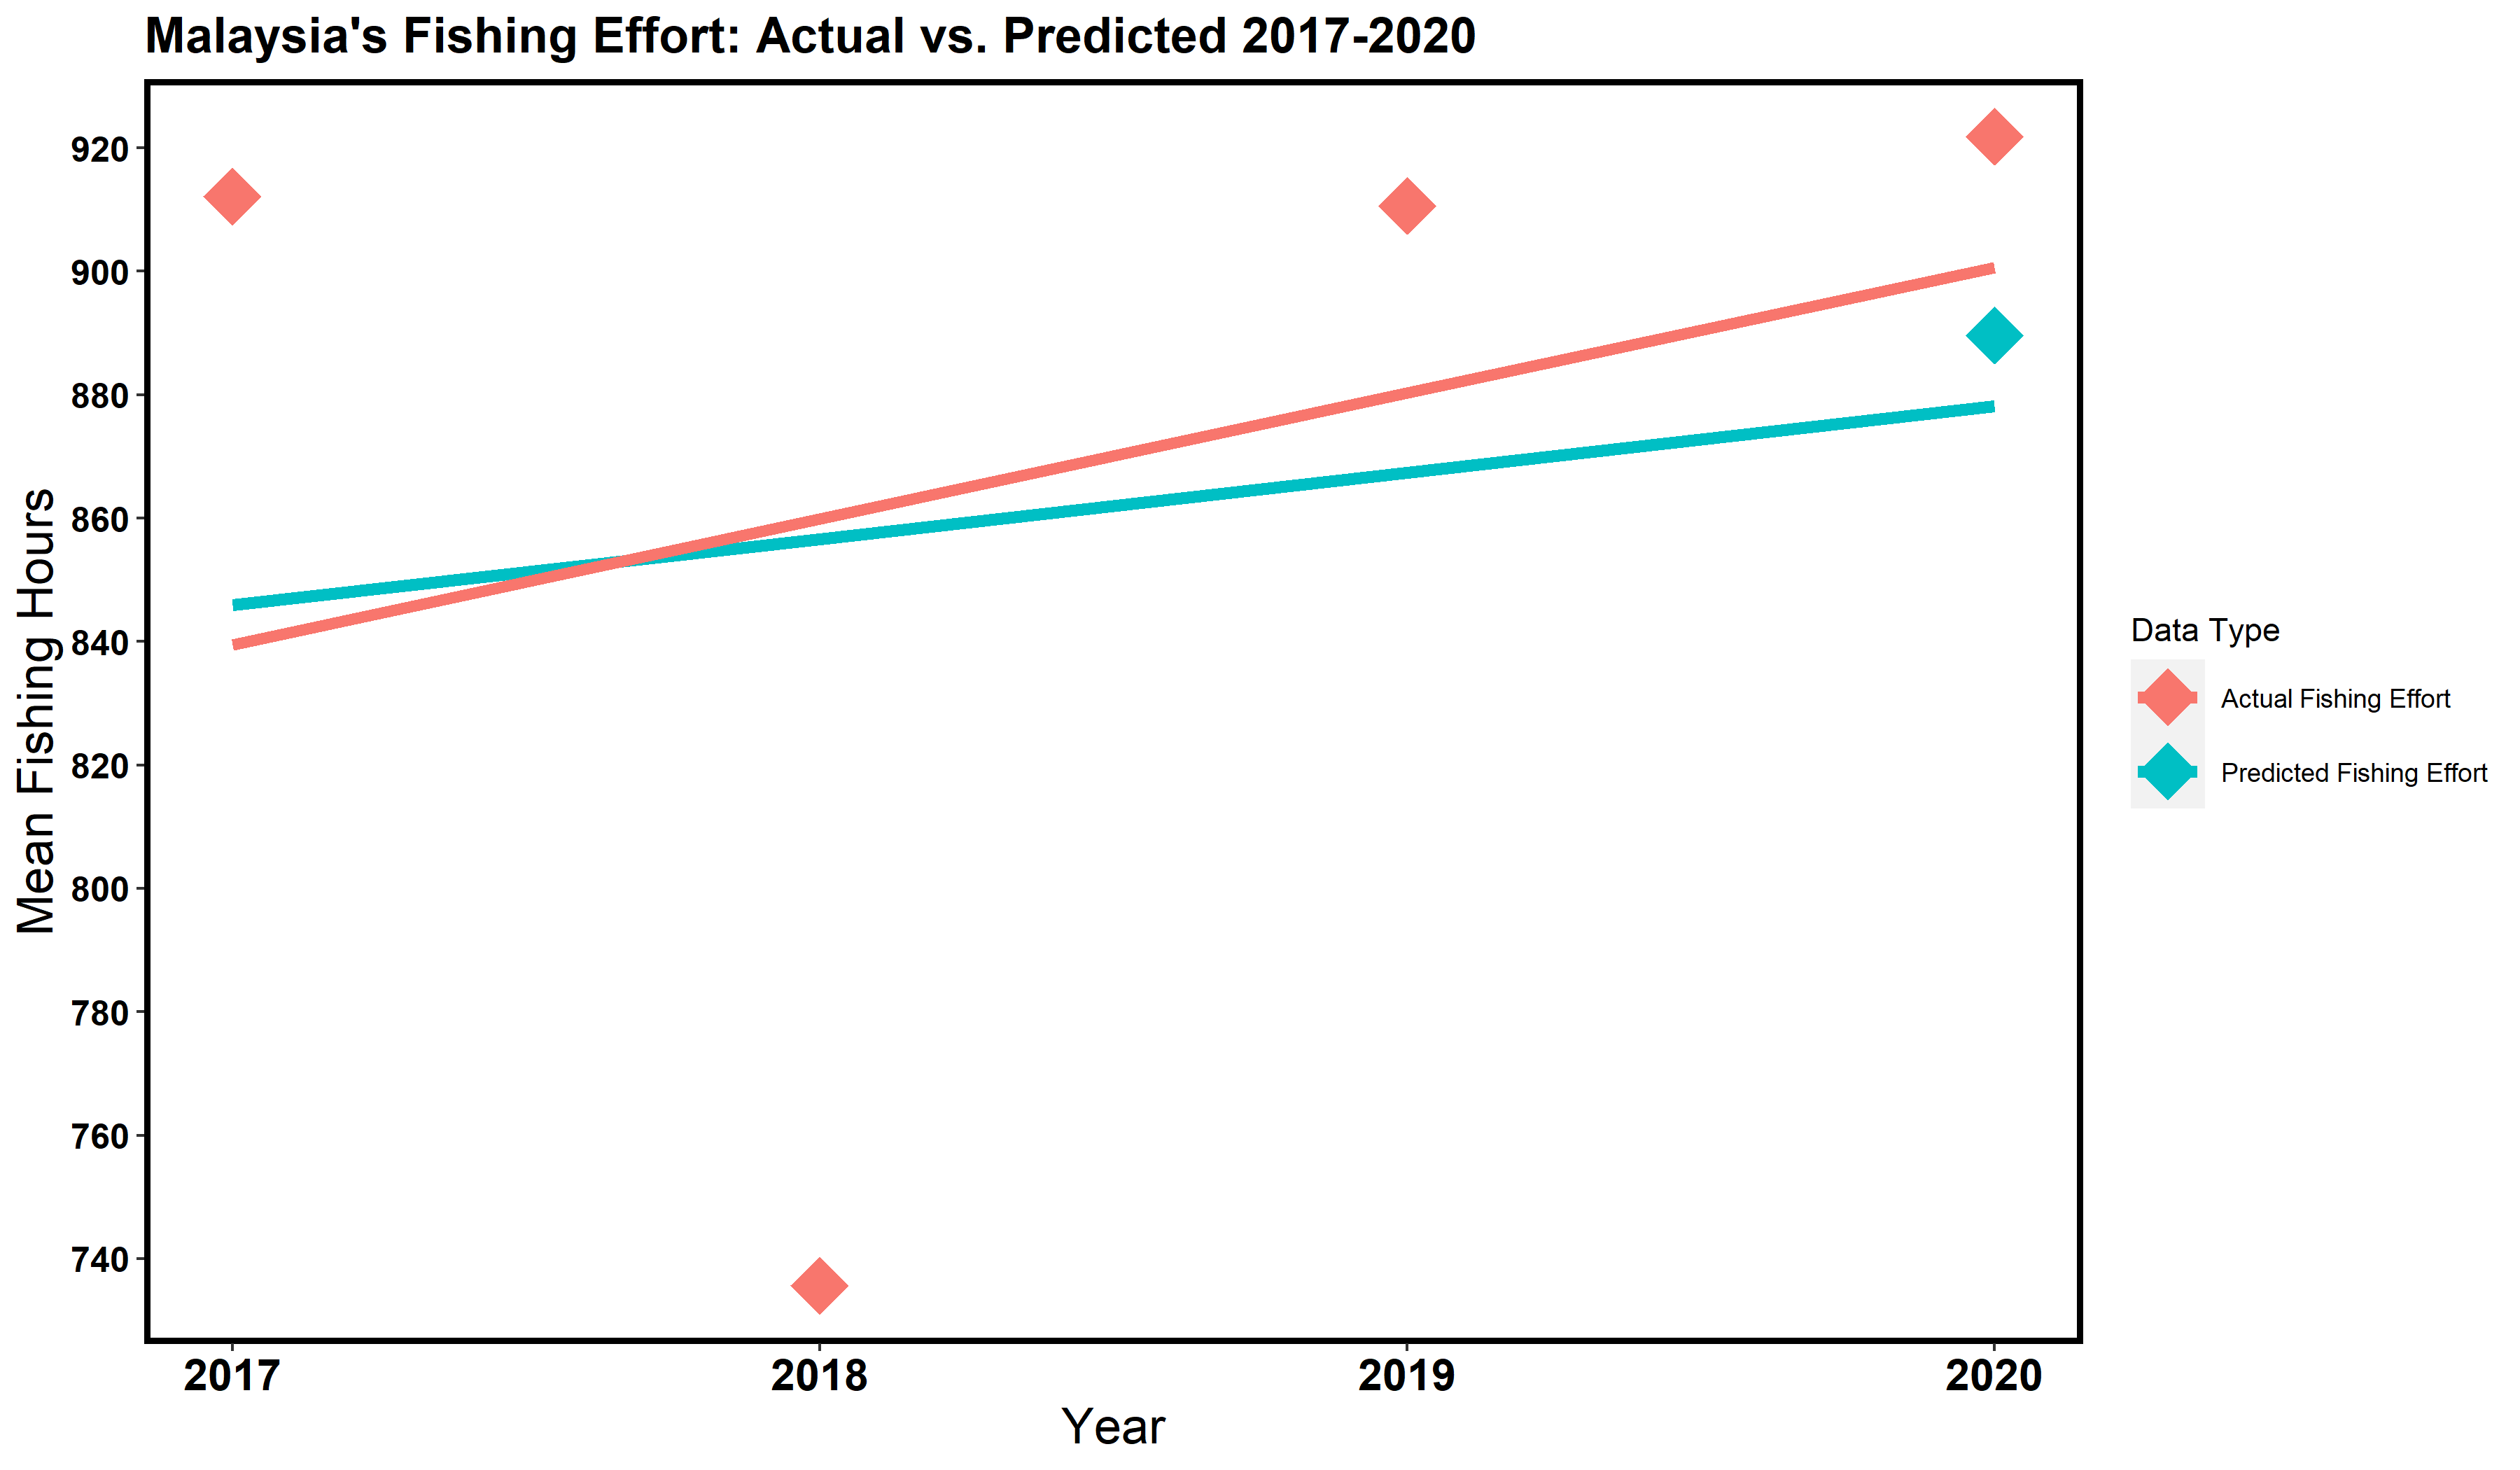
\includegraphics[width=0.7\textwidth,height=\textheight]{pictures/malaysia_fishing_effort_legend.png}
\caption{Malaysia's Fishing Effort: Actual vs Predicted 2017-2020}
\end{figure}

Malaysia increased their fishing effort in 2020 relative to their trend
leading up to 2020. Malaysia's fishing effort was approximately 922
hours, while our model predicted that this country would fish for
approximately 890 hours. This is a small margin.

\hypertarget{statistical-significance}{%
\subsubsection{Statistical
Significance}\label{statistical-significance}}

It's time to run a t-test to determine if there is a statistical
difference between the countries' predicted fishing effort in 2020 and
their actual fishing effort in 2020. A t-test is a handy tool in
statistics that reveals how significant the differences between groups
are. If the difference between the means of two groups could have easily
happened by chance, the p-value will be greater than 0.05 (which is the
standard threshold in statistics and environmental data science). If it
is highly unlikely (less than a 5\% chance) that a difference in means
at least this extreme could have occurred by chance, the p-value is less
than 0.05 and the results are considered statistically significant. A
statistically significant outcome allows us to reject our \textbf{null
hypothesis}.

\textbf{Null Hypothesis:} There is no difference between the predicted
country-specific predicted fishing effort in 2020 and the actual
country-specific fishing effort in 2020.
\[H_{0}: \mu_{predicted} - \mu_{actual} = 0\] \textbf{Alternative
Hypothesis:} There is a difference between the predicted
country-specific predicted fishing effort in 2020 and the actual
country-specific fishing effort in 2020. Because of the pandemic in
2020, I predict that fishing effort decreased, meaning that the actual
country-specific fishing effort is less than the predicted
country-specific fishing effort.
\[H_{A}: \mu_{predicted} - \mu_{actual} \neq 0\]

Don't forget to convert the data to \textbf{Tidy format} so we can run
the t-test!

\begin{Shaded}
\begin{Highlighting}[]
\NormalTok{comparison\_tidy }\OtherTok{\textless{}{-}}\NormalTok{ comparison\_2020\_pos }\SpecialCharTok{\%\textgreater{}\%} 
  \FunctionTok{pivot\_longer}\NormalTok{(}\AttributeTok{cols =}\NormalTok{ (}\StringTok{"actual\_2020"}\SpecialCharTok{:}\StringTok{"prediction\_2020"}\NormalTok{),}
               \AttributeTok{names\_to =} \StringTok{"actual\_or\_predicted"}\NormalTok{,}
               \AttributeTok{values\_to =} \StringTok{"mean\_effort"}\NormalTok{)}

\CommentTok{\# include this setting so the tiny p{-}value is not in scientific notation}
\FunctionTok{options}\NormalTok{(}\AttributeTok{scipen =} \DecValTok{999}\NormalTok{)}
\NormalTok{ttest }\OtherTok{=} \FunctionTok{t.test}\NormalTok{(mean\_effort }\SpecialCharTok{\textasciitilde{}}\NormalTok{ actual\_or\_predicted, }\AttributeTok{data =}\NormalTok{ comparison\_tidy, }\AttributeTok{conf.level =} \FloatTok{0.95}\NormalTok{)}
\NormalTok{ttest}
\end{Highlighting}
\end{Shaded}

\begin{verbatim}
## 
##  Welch Two Sample t-test
## 
## data:  mean_effort by actual_or_predicted
## t = -6.2015, df = 72.282, p-value = 0.0000000312
## alternative hypothesis: true difference in means between group actual_2020 and group prediction_2020 is not equal to 0
## 95 percent confidence interval:
##  -6761.425 -3472.097
## sample estimates:
##     mean in group actual_2020 mean in group prediction_2020 
##                      1406.727                      6523.488
\end{verbatim}

\begin{figure}
\centering
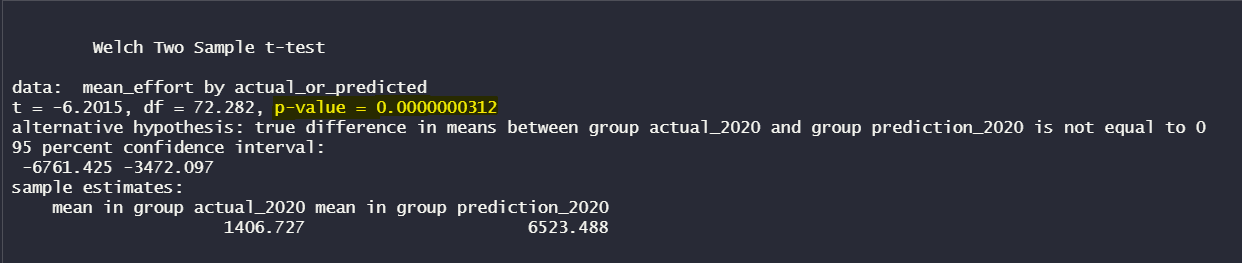
\includegraphics{pictures/ttest_highlighted.png}
\caption{\textbf{t-test output}}
\end{figure}

The p-value is 0.0000000312, and 0.0000000312 \textless{} 0.05, so we
can reject our null hypothesis that there is no difference between the
predicted country-specific predicted fishing effort in 2020 and the
actual country-specific fishing effort in 2020. Many countries clearly
changed their fishing effort in 2020 relative to their historical trend!

\hypertarget{summary-which-countries-increased-their-fishing-effort-during-the-pandemic-relative-to-their-trend-leading-up-to-2020}{%
\subsubsection{Summary: Which countries increased their fishing effort
during the pandemic, relative to their trend leading up to
2020?}\label{summary-which-countries-increased-their-fishing-effort-during-the-pandemic-relative-to-their-trend-leading-up-to-2020}}

To best visualize this fishing effort data in a table, we can color code
the countries that \textbf{increased} their fishing effort as red and
color the countries that \textbf{decreased} their fishing effort in
green.

\begin{Shaded}
\begin{Highlighting}[]
\CommentTok{\# convert the comparison\_tidy data to a table}

\CommentTok{\# first, rearrange the columns}
\NormalTok{comparison\_data\_rearranged }\OtherTok{\textless{}{-}}\NormalTok{ comparison\_tidy[, }\FunctionTok{c}\NormalTok{(}\DecValTok{1}\NormalTok{, }\DecValTok{5}\NormalTok{, }\DecValTok{4}\NormalTok{, }\DecValTok{2}\NormalTok{, }\DecValTok{3}\NormalTok{)]}

\CommentTok{\# reduce the amount of rows to 1 per country, and select just the rows of interest for the table}
\NormalTok{delete }\OtherTok{\textless{}{-}} \FunctionTok{seq}\NormalTok{(}\DecValTok{1}\NormalTok{, }\FunctionTok{nrow}\NormalTok{(comparison\_data\_rearranged), }\DecValTok{2}\NormalTok{)}
\NormalTok{comparison\_rearranged\_simplified }\OtherTok{\textless{}{-}}\NormalTok{ comparison\_data\_rearranged[ delete ,]}
\NormalTok{comparison\_rearranged\_simplified }\OtherTok{\textless{}{-}}\NormalTok{ comparison\_rearranged\_simplified }\SpecialCharTok{\%\textgreater{}\%} 
  \FunctionTok{select}\NormalTok{(flag\_gfw, difference\_a\_minus\_p, change\_direc)}

\NormalTok{good\_bad\_table }\OtherTok{\textless{}{-}}\NormalTok{ comparison\_rearranged\_simplified }\SpecialCharTok{\%\textgreater{}\%} 
  \FunctionTok{gt}\NormalTok{() }\SpecialCharTok{\%\textgreater{}\%}
  \FunctionTok{tab\_header}\NormalTok{(}
    \AttributeTok{title =} \FunctionTok{md}\NormalTok{(}\StringTok{"**Which countries increased or decreased 2020 fishing effort relative to their trend?**"}\NormalTok{)}
\NormalTok{  ) }\SpecialCharTok{\%\textgreater{}\%}
  \FunctionTok{fmt\_passthrough}\NormalTok{(}
    \AttributeTok{columns =} \FunctionTok{c}\NormalTok{(flag\_gfw)}
\NormalTok{  ) }\SpecialCharTok{\%\textgreater{}\%}
  \FunctionTok{fmt\_number}\NormalTok{(}
  \AttributeTok{columns =} \FunctionTok{c}\NormalTok{(difference\_a\_minus\_p)}
\NormalTok{  ) }\SpecialCharTok{\%\textgreater{}\%}
  \FunctionTok{fmt\_passthrough}\NormalTok{(}
    \AttributeTok{columns =} \FunctionTok{c}\NormalTok{(change\_direc)}
\NormalTok{  ) }\SpecialCharTok{\%\textgreater{}\%}
  \FunctionTok{cols\_label}\NormalTok{(}\AttributeTok{flag\_gfw =} \StringTok{"Country Code"}\NormalTok{ , }
           \AttributeTok{difference\_a\_minus\_p =} \StringTok{"Difference: Actual {-} Prediction"}\NormalTok{,}
           \AttributeTok{change\_direc =} \StringTok{"Fishing Effort Relative to Trend"}\NormalTok{) }\SpecialCharTok{\%\textgreater{}\%} 
  \FunctionTok{tab\_style}\NormalTok{(}
    \AttributeTok{style =} \FunctionTok{list}\NormalTok{(}
      \FunctionTok{cell\_fill}\NormalTok{(}\AttributeTok{color =} \StringTok{"chartreuse2"}\NormalTok{),}
      \FunctionTok{cell\_text}\NormalTok{(}\AttributeTok{weight =} \StringTok{"bold"}\NormalTok{)}
\NormalTok{      ),}
    \AttributeTok{locations =} \FunctionTok{cells\_body}\NormalTok{(}
      \AttributeTok{columns =} \FunctionTok{c}\NormalTok{(flag\_gfw, difference\_a\_minus\_p, change\_direc),}
      \AttributeTok{rows =}\NormalTok{ change\_direc }\SpecialCharTok{==} \StringTok{"fished LESS than trend"}\NormalTok{)}
\NormalTok{  ) }\SpecialCharTok{\%\textgreater{}\%} 
  \FunctionTok{tab\_style}\NormalTok{(}
    \AttributeTok{style =} \FunctionTok{list}\NormalTok{(}
      \FunctionTok{cell\_fill}\NormalTok{(}\AttributeTok{color =} \StringTok{"brown2"}\NormalTok{),}
      \FunctionTok{cell\_text}\NormalTok{(}\AttributeTok{weight =} \StringTok{"bold"}\NormalTok{)}
\NormalTok{      ),}
    \AttributeTok{locations =} \FunctionTok{cells\_body}\NormalTok{(}
      \AttributeTok{columns =} \FunctionTok{c}\NormalTok{(flag\_gfw, difference\_a\_minus\_p, change\_direc),}
      \AttributeTok{rows =}\NormalTok{ change\_direc }\SpecialCharTok{==} \StringTok{"fished MORE than trend"}\NormalTok{)}
\NormalTok{  ) }\SpecialCharTok{\%\textgreater{}\%} 
  \FunctionTok{tab\_source\_note}\NormalTok{(}\AttributeTok{source\_note =} \StringTok{"Data Source: Global Fishing Watch: https://globalfishingwatch.org/datasets{-}and{-}code/"}\NormalTok{) }\SpecialCharTok{\%\textgreater{}\%}
  \FunctionTok{opt\_align\_table\_header}\NormalTok{(}\AttributeTok{align =} \StringTok{"center"}\NormalTok{) }\SpecialCharTok{\%\textgreater{}\%} 
  \FunctionTok{cols\_width}\NormalTok{(}
\NormalTok{    flag\_gfw }\SpecialCharTok{\textasciitilde{}} \FunctionTok{px}\NormalTok{(}\DecValTok{150}\NormalTok{),}
\NormalTok{    difference\_a\_minus\_p }\SpecialCharTok{\textasciitilde{}} \FunctionTok{px}\NormalTok{(}\DecValTok{150}\NormalTok{),}
\NormalTok{    change\_direc }\SpecialCharTok{\textasciitilde{}} \FunctionTok{px}\NormalTok{(}\DecValTok{220}\NormalTok{)}
\NormalTok{  ) }\SpecialCharTok{\%\textgreater{}\%} 
  \FunctionTok{cols\_align}\NormalTok{(}\AttributeTok{align =} \StringTok{"center"}\NormalTok{)}

\NormalTok{good\_bad\_table}
\end{Highlighting}
\end{Shaded}

\captionsetup[table]{labelformat=empty,skip=1pt}
\begin{longtable}{ccc}
\caption*{
{\large \textbf{Which countries increased or decreased 2020 fishing effort relative to their trend?}}
} \\ 
\toprule
Country Code & Difference: Actual - Prediction & Fishing Effort Relative to Trend \\ 
\midrule
AGO & $-18,839.60$ & fished LESS than trend \\ 
ARG & $-1,589.04$ & fished LESS than trend \\ 
AUS & $-2,912.65$ & fished LESS than trend \\ 
BEL & $1,957.92$ & fished MORE than trend \\ 
BHR & $-1,096.14$ & fished LESS than trend \\ 
CHN & $483.96$ & fished MORE than trend \\ 
CIV & $1,716.01$ & fished MORE than trend \\ 
COL & $-7,640.26$ & fished LESS than trend \\ 
CUW & $-679.30$ & fished LESS than trend \\ 
CYP & $-893.07$ & fished LESS than trend \\ 
DEU & $-1,132.22$ & fished LESS than trend \\ 
DNK & $-1,138.36$ & fished LESS than trend \\ 
DZA & $-966.74$ & fished LESS than trend \\ 
FIN & $-1,181.76$ & fished LESS than trend \\ 
FLK & $-8,901.31$ & fished LESS than trend \\ 
FRA & $-3,911.13$ & fished LESS than trend \\ 
FRO & $-17,991.09$ & fished LESS than trend \\ 
FSM & $-10,412.30$ & fished LESS than trend \\ 
GBR & $696.23$ & fished MORE than trend \\ 
GNB & $-2,829.85$ & fished LESS than trend \\ 
GRC & $-1,090.50$ & fished LESS than trend \\ 
GRL & $1,740.20$ & fished MORE than trend \\ 
GTM & $-9,408.47$ & fished LESS than trend \\ 
HKG & $-1,135.99$ & fished LESS than trend \\ 
HND & $499.66$ & fished MORE than trend \\ 
HRV & $-1,312.42$ & fished LESS than trend \\ 
IND & $-2,115.41$ & fished LESS than trend \\ 
IRL & $-1,781.87$ & fished LESS than trend \\ 
IRN & $-10,708.15$ & fished LESS than trend \\ 
ITA & $-455.14$ & fished LESS than trend \\ 
JPN & $-7,306.61$ & fished LESS than trend \\ 
KIR & $-22,066.68$ & fished LESS than trend \\ 
KOR & $-1,961.90$ & fished LESS than trend \\ 
LBR & $-3,835.59$ & fished LESS than trend \\ 
LTU & $-965.70$ & fished LESS than trend \\ 
LVA & $-3,866.25$ & fished LESS than trend \\ 
MEX & $-183.88$ & fished LESS than trend \\ 
MHL & $-4,459.09$ & fished LESS than trend \\ 
MLT & $-3,403.21$ & fished LESS than trend \\ 
MOZ & $-30,463.68$ & fished LESS than trend \\ 
MRT & $-3,967.54$ & fished LESS than trend \\ 
MUS & $-4,556.00$ & fished LESS than trend \\ 
MYS & $32.19$ & fished MORE than trend \\ 
NCL & $-16,767.26$ & fished LESS than trend \\ 
NIC & $-12,025.34$ & fished LESS than trend \\ 
NLD & $-5,488.85$ & fished LESS than trend \\ 
NOR & $-637.39$ & fished LESS than trend \\ 
NRU & $-23,059.46$ & fished LESS than trend \\ 
NZL & $-3,033.13$ & fished LESS than trend \\ 
PHL & $-4,969.43$ & fished LESS than trend \\ 
PNG & $-6,850.56$ & fished LESS than trend \\ 
POL & $-2,654.60$ & fished LESS than trend \\ 
PRT & $-5,154.99$ & fished LESS than trend \\ 
PYF & $-14,175.81$ & fished LESS than trend \\ 
ROU & $-7,758.79$ & fished LESS than trend \\ 
RUS & $-6,501.55$ & fished LESS than trend \\ 
SAU & $-1,057.84$ & fished LESS than trend \\ 
SEN & $1,264.19$ & fished MORE than trend \\ 
SLV & $-4,308.69$ & fished LESS than trend \\ 
SVN & $-6,581.25$ & fished LESS than trend \\ 
SYC & $-7,965.57$ & fished LESS than trend \\ 
TCA & $-2,742.51$ & fished LESS than trend \\ 
TUR & $235.48$ & fished MORE than trend \\ 
TUV & $-20,921.43$ & fished LESS than trend \\ 
UKR & $-9,779.68$ & fished LESS than trend \\ 
UNK & $327.21$ & fished MORE than trend \\ 
URY & $-1,521.12$ & fished LESS than trend \\ 
USA & $-148.03$ & fished LESS than trend \\ 
VEN & $-2,640.55$ & fished LESS than trend \\ 
VUT & $-9,212.82$ & fished LESS than trend \\ 
ZAF & $872.42$ & fished MORE than trend \\ 
 \bottomrule
\end{longtable}
\begin{minipage}{\linewidth}
Data Source: Global Fishing Watch: https://globalfishingwatch.org/datasets-and-code/\\ 
\end{minipage}

\begin{Shaded}
\begin{Highlighting}[]
\FunctionTok{gtsave}\NormalTok{(}\AttributeTok{data =}\NormalTok{ good\_bad\_table, }\AttributeTok{filename =} \StringTok{"good\_bad\_table\_correct.png"}\NormalTok{, }\AttributeTok{path =} \FunctionTok{here}\NormalTok{())}
\end{Highlighting}
\end{Shaded}

\includegraphics{to_pdf_files/figure-latex/unnamed-chunk-9-1}

\begin{figure}
\centering
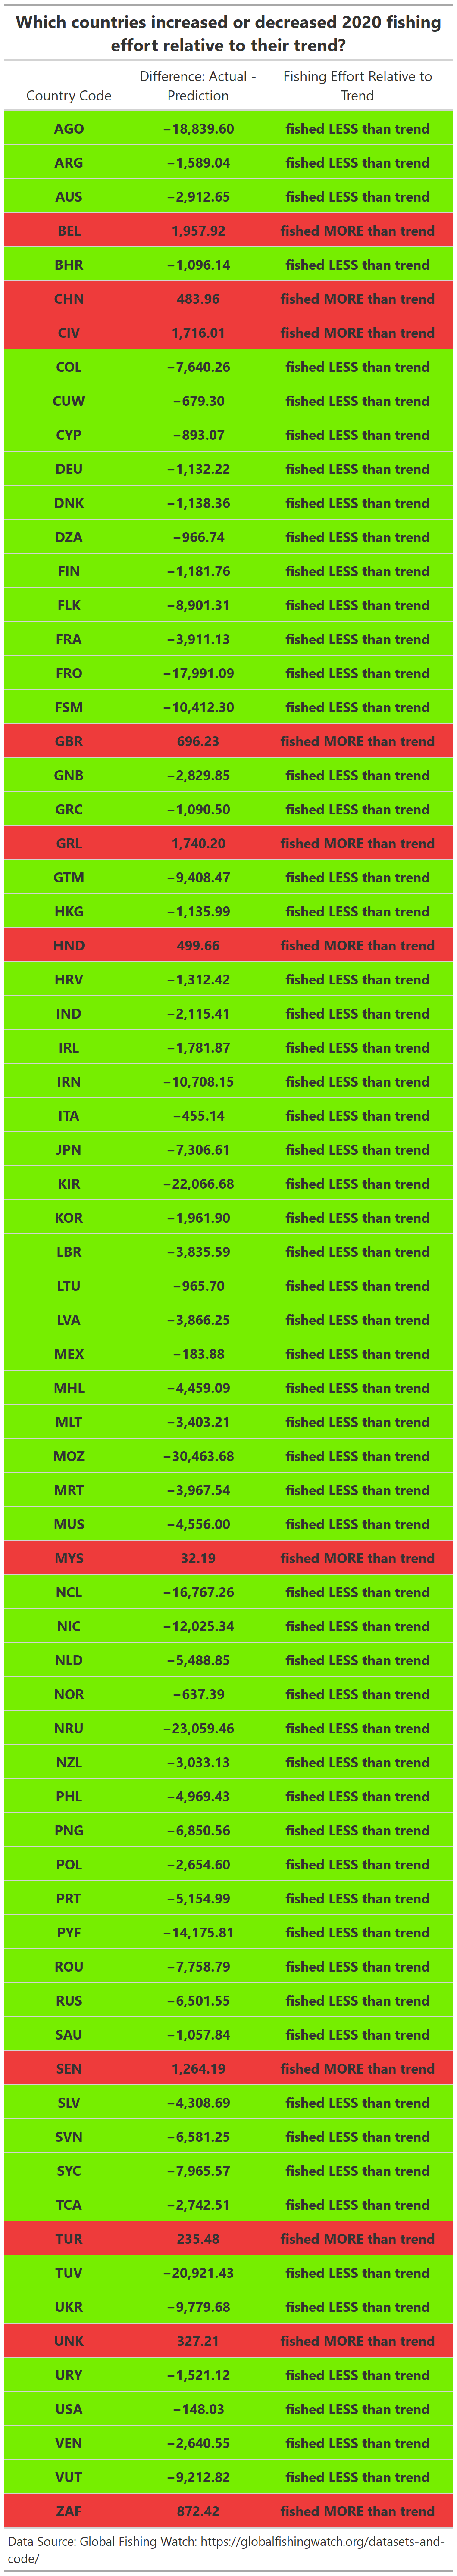
\includegraphics{pictures/good_bad_table_correct.png}
\caption{Differences between actual 2020 fishing effort and predicted
2020 fishing effort by country}
\end{figure}

This color-coded table reveals that 85\% of the countries included in
this analysis \emph{decreased} their fishing effort during the Covid-19
pandemic in 2020 relative to their fishing trend leading up to 2020,
while 15\% of the countries included in this analysis \emph{increased}
their fishing effort. The vast majority of countries' fishing sectors
seemed to follow the same stay-at-home order that was enforced across
the globe. While this may have had a detrimental impact on the global
fish economy, hopefully the marine fish populations we able to recover
and thrive during this period of reprieve from predation. The results of
my statistical analysis match the conclusion of a 2021 scientific study
investigating the change in marine recreational fishing activity during
the first year of the pandemic (5).

\hypertarget{future-steps}{%
\subsubsection{Future Steps}\label{future-steps}}

In order to make this analysis more robust in the future, I recommend
using more than 3 years of fishing effort data to produce a more
accurate linear model. Additionally, I would recommend using a different
statistical approach instead of iterating a for loop over each country's
fishing effort data, because this method did not produce a very accurate
linear regression. Lastly, I recommend running this analysis on fishing
effort data from other sources in addition to Global Fishing Watch's
data. This will provide certainty that the data is accurate and the
results are reproducible.

Thank you for reading my statistical review of global fishing effort
during the 2020 Covid-19 pandemic. I hope you have been inspired to run
your own linear regressions, t-tests, and create visualizations that
help communicate trends in environmental data science. Please feel free
to contact me at
\href{mailto:jscohen@ucsb.edu}{\nolinkurl{jscohen@ucsb.edu}} with any
questions, comments, or suggestions. You may also create issues or pull
requests for this analysis through GitHub (repository linked below).

\hypertarget{data-availability}{%
\paragraph{Data Availability}\label{data-availability}}

The data used in this analysis is openly available, but the user must
make a free account on the Global Fishing watch website, which can be
accessed through this live link:\\
\href{https://globalfishingwatch.org/data-download/datasets/public-fishing-effort}{Global
Fishing Watch Datasets and Code}\\

\hypertarget{github-repository}{%
\paragraph{GitHub Repository}\label{github-repository}}

\href{https://github.com/julietcohen/fishing_effort}{julietcohen's
GitHub Repository: see to\_pdf.Rmd}

\hypertarget{acknowledgements}{%
\paragraph{Acknowledgements:}\label{acknowledgements}}

\begin{itemize}
\tightlist
\item
  I would like to acknowledge Dr.~Tamma Carleton, my professor in
  Statistics for Environmental Data Science at the U.C. Santa Barbara
  Bren School for Environmental Science and Management, for all her
  support throughout this project and this quarter.\\
\item
  I would also like to thank my peers in the Master of Environmental
  Data Science Program for being so open to collaboration and supporting
  each other with resources, programming tools, and open-source
  science.\\
\item
  Lastly, I would like to thank Global Fishing Watch for inspiring me to
  give a hoot about global fishing effort by country, and for providing
  the data that made this project possible.
\end{itemize}

\hypertarget{resources-live-links}{%
\paragraph{Resources (live links):}\label{resources-live-links}}

\begin{enumerate}
\def\labelenumi{\arabic{enumi}.}
\tightlist
\item
  \href{https://globalfishingwatch.org/map/?latitude=19\&longitude=-30\&zoom=1.5\&start=2021-08-26T23\%3A00\%3A00.000Z\&end=2021-11-27T00\%3A00\%3A00.000Z}{World
  Maps of Fishing Activity: Pictures 1 \& 2 - Global Fishing Watch}\\
\item
  \href{https://globalfishingwatch.org/carrier-portal/?latitude=12.7069821\&longitude=19.1776829\&zoom=1.1903704\&layer\%5B0\%5D=encounter\&layer\%5B1\%5D=cp_rfmo\&layer\%5B2\%5D=cp_next_port\&dataset=carriers:v20211001\&tab=flags}{World
  Map of Fishing by Country: Picture 3 - Global Fishing Watch}\\
\item
  \href{https://globalfishingwatch.org/data-download/datasets/public-fishing-effort}{Global
  Fishing Watch: Datasets and Code, Fishing effort data}\\
  note: Users must make a free account in order to access datasets\\
\item
  \href{https://www.sciencedirect.com/science/article/pii/S0165783610002754?casa_token=o12VmHrPGdkAAAAA:Y0YdOekq7DtNi7wVL0WNShArvCUl6x_S5yURGiEVKNe95eaYAM9y4GP-uqr1bl1bp71A8rNgWj4}{Global
  Fishing Effort (1950--2010): Trends, Gaps, and Implications.}\\
  Anticamara, J. A., R. Watson, A. Gelchu, and D. Pauly. ``Global
  Fishing Effort (1950--2010): Trends, Gaps, and Implications.''
  Fisheries Research 107, no. 1 (2011): 131--36.
  \url{https://doi.org/10.1016/j.fishres.2010.10.016./}
\item
  \href{https://www.frontiersin.org/articles/10.3389/fmars.2021.735741/full}{First
  Assessment of the Impacts of the COVID-19 Pandemic on Global Marine
  Recreational Fisheries.}:\\
  Pita, Pablo, Gillian B. Ainsworth, Bernardino Alba, Antônio B.
  Anderson, Manel Antelo, Josep Alós, Iñaki Artetxe, et al.~``First
  Assessment of the Impacts of the COVID-19 Pandemic on Global Marine
  Recreational Fisheries.'' Frontiers in Marine Science 8 (2021): 1533.
  \url{https://doi.org/10.3389/fmars.2021.735741./}
\item
  \href{http://www.seafdec.org/fisheries-country-profile-malaysia/\#:~:text=Fish\%20trade\%20is\%20valued\%20at,56.8\%20kg\%2Fperson\%2Fyear.\&text=Marine\%20capture\%20fisheries\%20is\%20the,providing\%20work\%20to\%20132\%2C305\%20people.}{Malaysia's
  Fisheries Economy}\\
\item
  \href{https://www.google.com/maps/place/Malaysia/@4.1279224,105.1196274,6z/data=!3m1!4b1!4m5!3m4!1s0x3034d3975f6730af:0x745969328211cd8!8m2!3d4.210484!4d101.975766}{Google
  Maps: Malaysia}\\
\item
  \href{https://en.wikipedia.org/wiki/Ocean_fisheries\#:~:text=The\%20ocean\%20has\%20some\%20of,hake\%2C\%20herring\%2C\%20and\%20mackerel.}{Wikipedia:
  Top Marine Fisheries Species Captured}
\end{enumerate}

Distill is a publication format for scientific and technical writing,
native to the web.

Learn more about using Distill at
\url{https://rstudio.github.io/distill}.

\end{document}
